\documentclass[11pt,oneside]{book}
\usepackage{natbib}
\usepackage{color}
\usepackage{amsmath}
\usepackage{amssymb}
\usepackage{graphicx}
\usepackage{epsfig}
\usepackage{amsmath}
\usepackage{amssymb}
\usepackage{shadow}
\usepackage{tablefootnote}
\usepackage{tabto}
\usepackage{tikz}
\usepackage{graphicx,wrapfig,lipsum}
\usepackage{caption}
\usepackage{subcaption}
\usepackage{esvect}
\usepackage{hyperref}
\usepackage{booktabs}
\usepackage{Myfullpage}
\usepackage{placeins}
%\usepackage{fullname}
\usepackage{times}
\usepackage{covington}
%\usepackage{mathbbol}
\usepackage{amsthm}
\usepackage{amssymb}
\usepackage{url}

%\usepackage{txfonts}
\usepackage{%
  pstricks,
  pst-node}
\usepackage{fancyhdr}
\usepackage{amssymb,amsmath}
\usepackage{epsfig,graphics}
\usepackage{llncsdoc}
\usepackage{enumerate}
\usepackage{amsmath}
\usepackage{algorithm,algorithmic}
\renewcommand{\algorithmicrequire}{\textbf{Inputs:}}
\renewcommand{\algorithmicensure}{\textbf{Outputs:}}

% PSTricks settings and definitions
\let\Oldsection\section
\renewcommand{\section}{\FloatBarrier\Oldsection}

\let\Oldsubsection\subsection
\renewcommand{\subsection}{\FloatBarrier\Oldsubsection}

\let\Oldsubsubsection\subsubsection
\renewcommand{\subsubsection}{\FloatBarrier\Oldsubsubsection}

\psset{nodesep=3pt}
% a state of an automaton
\newcommand{\state}[2]{\circlenode{#1}{#2}}
% an initial state: shaded circle
\newcommand{\istate}[2]{\circlenode[fillstyle=solid,fillcolor=lightgray]{#1}{#2}}
% a final state: double circles with a small separating distance
\newcommand{\fstate}[2]{\circlenode[framesep=0pt]{#1}{\pscirclebox[framesep=1pt]{#2}}}
% an initial and final state
\newcommand{\ifstate}[2]{\circlenode[framesep=0pt]{#1}{\pscirclebox[fillstyle=solid,fillcolor=lightgray,framesep=1pt]{#2}}}
% an arc. parameters:
% 1 (optional): 2 angles
% 2: source node; 3: target node; 4: label.
\newcommand{\trans}[4][angleA=0,angleB=180]{\nccurve[#1]{->}{#2}{#3}\Aput{#4}}
\newcommand{\transdash}[4][angleA=0,angleB=180,linestyle=dashed]{\nccurve[#1]{->}{#2}{#3}\Aput{#4}}
\newcommand{\transdot}[4][angleA=0,angleB=180,linestyle=dotted]{\nccurve[#1]{->}{#2}{#3}\Aput{#4}}
\renewcommand{\baselinestretch}{1.67}
\newcommand{\minispace}{\mbox{\hspace{1mm}}}
\newcommand{\smallspace}{\mbox{\hspace{3mm}}}
\newcommand{\bigspace}{\mbox{\hspace{10mm}}}
\newcommand{\textnl}{\textsl}
\newcommand{\naturals}{\mathbb{N}}
\newtheorem{definition}{Definition}[chapter]
\newtheorem{proposition}{Proposition}[chapter]
\newtheorem{lemma}{Lemma}[chapter]
\newtheorem{exa}{Example}[chapter]
\newtheorem{observation}{Observation}[chapter]
\newtheorem{claim}{Claim}[chapter]
\newtheorem{corollary}{Corollary}[chapter]
\newtheorem{theorem}{Theorem}[chapter]
\newcommand{\comment}[1]{}

\newcommand{\edge}[3]{{#1}\buildrel{#2}\over\longrightarrow{#3}}
\newcommand{\transition}{{\bf M}}

\def\ignore#1{}

\begin{document}
\date{\today\\v1.3}
\title{\Huge{The ecology of Web browser}
                \huge
             \\[10mm] Sela Ferdman
             \\[25mm] \Large THESIS SUBMITTED IN PARTIAL FULFILLMENT OF THE
             \\       REQUIREMENTS FOR THE MASTER DEGREE
             \\[15mm] University of Haifa
             \\       Faculty of Social Sciences
             \\       Department of Computer Sciences
             \\[10mm] March, 2015
}
\date{\today\\v1.3}
\maketitle{}

\pagestyle{plain}
\pagenumbering{Roman}

\begin{center}
\Huge
     The ecology of Web browser
\huge
\\[10mm] By: Sela Ferdman
\\[3mm] Supervised By: Dr. Einat Minkov and Dr. Ron Bekkerman
\Large
\\ [10mm]THESIS SUBMITTED IN PARTIAL FULFILLMENT OF THE
\\ REQUIREMENTS FOR THE MASTER DEGREE
\\ [10mm]University of Haifa
\\ [1mm]Faculty of Social Sciences
\\ [1mm]Department of Computer Sciences
\\ [3mm]March, 2015
\\ [8mm] Approved by:
$\underline{\bigspace\bigspace\bigspace\bigspace\bigspace\bigspace\bigspace\bigspace}$
   \bigspace    Date:$\underline{\bigspace\bigspace}$
\\ (supervisor)\bigspace
\\ [3mm]Approved by:
$\underline{\bigspace\bigspace\bigspace\bigspace\bigspace\bigspace\bigspace\bigspace}$
   \bigspace    Date:$\underline{\bigspace\bigspace}$
\\ (Chairman of  M.Sc Committee) \bigspace

\end{center}

\iffalse
\chapter*{}
\begin{center}
\LARGE{Acknowledgment}
\end{center}
\fi


\chapter*{}

\addcontentsline{toc}{chapter}{Abstract}
\begin{center}
\iffalse
\huge{Learning Context Selection Models for Knowledge-based WSD}
\\ [10mm] Sela Ferdman
\fi
\huge{Abstract}
\end{center}


TBA

\tableofcontents

\listoffigures
\addcontentsline{toc}{chapter}{List of Figures}
\listoftables
\addcontentsline{toc}{chapter}{List of Tables}

\chapter{Introduction}
\thispagestyle{empty}
\pagenumbering{arabic}

Web browsers, a software application for retrieving and presenting resources on the World Wide Web, have become a major part of our computer ecosystem. In fact, some recent operating systems are based entirely on browsers (e.g., ChromeOS by Google\footnote{\url{http://www.chromium.org/chromium-os}}). Browser extensions (also called add-ons) are computer programs, which allow the user to customize a browser to meet his or her needs. These extensions (as the name suggests) extend, improve and personalize browser capabilities. An extension was developed, for example, that provides visually impaired users with access to the content of bar charts on the Web \cite{elzer2007browser}. Another example browser add-on addresses security concerns, transparently producing a different password for each Website, and by that defending the user against password phishing and other attacks \citep{ross2005stronger}. A great number of extensions are installed by users on a daily basis nowadays. It was reported that more than 750 million (non-unique) extensions were downloaded and installed by users of Google Chrome alone as of June 2012\footnote{\url{http://www.medianama.com/2012/06/223-the-lowdown-google-io-2012-day-2-310m-chrome-users-425m-gmail-more}}.  Toolbars are considered to be a particular kind of a browser extension. A browser toolbar is a GUI widget, which typically resides in the upper part of the browser's window. All major Web browsers support toolbar development as means of extending the browser's GUI and functionality. While browser extensions in general, and toolbars in particular, may be installed following an explicit request by the user, these add-ons are often `silently' installed by a third party as the user downloads some other program from the Web, or add-ons may be included in a 'software bundle'. There are several reasons why software companies are interested in having specific toolbars installed on the user's machine. First, a special characteristic of toolbars is that they are often used for collecting information about the browsing history of the user (e.g., Yahoo! Toolbar \citep{kumar2010characterization}). In addition, it is often the case that once the toolbars are installed, all user searches are directed to some dedicated search portal (e.g. MyWebSearch.com). The company which owns the Website (and typically also the toolbar) typically receives payments from ad providers (primary ad providers today are Google and Yahoo!), when user clicks on ads presented. In fact, this model is used extensively nowadays to generate revenue by software companies, which otherwise distribute freeware products \citep{leontiadis2012don}. For example, 45\% of AVG Technologies sales were due to its browser toolbar\footnote{\url{http://seekingalpha.com/article/1147451-avg-feb-1st-google-policy-updates-threaten-avg-s-growth-engine-signals-steep-downside}}.  It was recently estimated that Google, the biggest Web advertising firm, may lose \$1.3 billion in 2013 revenue  due to its toolbar policy changes, which might cause some of the companies to shift to its competitors\footnote{\url{http://finance.yahoo.com/news/google-may-miss-2013-revenue-113926474.html}}\footnote{\url{https://support.google.com/adwordspolicy/answer/50423?hl=en}} . Importantly, a user serves as a source of income to the installing party as long as he or she actively uses the toolbar, where users may choose to remove the software from their system anytime. The ability to estimate the period of toolbar ‘survival’ is therefore critical in considering a business model for companies that distribute their software as freeware, counting on revenue generated due to installed toolbars. For example, when a user installs Babylon's translation software , he is offered to install also AVG toolbar, where AVG pays Babylon for these installations. If AVG could estimate whether a specific user would keep its toolbar, it could apply a differential payment model to Babylon according to estimated 'user value'.  In the proposed research, we will consider a large-scale authentic data that tracks browser extensions installed at users' machines on a daily basis. In addition to daily 'reporting', events of adding new browser toolbars are explicitly recorded. Removal
of toolbars can be inferred. We are interested in exploring trends in this large-scale data, and in answering specific questions, such as 'can one predict if a particular add-on survives on the user's machine
more than K days'. Providing a prediction model of good quality in response to this question is highly valuable to the industry, as discussed above. We will explore machine learning techniques to create prediction models of interest. While many academic studies have used information about user environment towards the creation of user
profiles and personalization of software services, there is no previous research, to the best of our knowledge, which used information about user browser extensions to similarly model user behavior. We will examine the hypothesis by which the existence of an extension on a user’s computer reflects something about the user's
application download history, as well as about his or her general preferences. Specifically, we will evaluate whether clustering users using the underlying data allows one to improve prediction of future behavior. The main research questions and goals are stated in Section 3. An overview of related literature is given below. In addition to previous works on user profiling, we discuss recent learning methods used in large-scale recommendation systems, relating in detail to clustering techniques, which are used to alleviate data sparsity
issues. Finally, descriptions of the prediction models that we plan to use, and an account of the special characteristics and challenges involved with the dataset.

[RON: The outline of our findings: In first half of the thesis, we operate on the user level. We use historical data to identify highly probable addons given the collection of addons of a specific user. In the second half of the thesis, we abstract the user data into insights at the addon company level. We identify which addon companies tend to coexist or clash with each other. Both analysis (user-level and company-level) can be used for prediction purposes. Given a specific collection of addons of a specific user, we can make a prediction which addons might get installed on this user's machine. Given two addon companies that were identified as partnering / competing with each other, we can predict their behavior in the future as their addons are evolving.]

[RON: a paragraph about human factor. After all, we are mostly interested in the user who owns the machine and either installs lots of garbage on it or tries to keep it as clean as possible. Who's is more important here - the user who cares about his/her machine hygiene or the bunch of companies that are trying to push stuff on the user's machine? Who's winning?]

[RON: the term ``computer virus'' has existed for a while - the connection between a hardware system (a computer) with a biological system is quite intuitive. However, we go far beyond this - we're investigating biological \_processes\_ in an artificial environment, which sounds pretty novel]

\section{Main Contributions}
\label{sub:contributions}
The main contributions of this work are the following:
\begin{itemize}
\renewcommand{\labelitemi}{$\bullet$} 
\item 
\end{itemize}

\section{Roadmap}
\label{sub:roadmap}


\chapter{Related Research}
\label{sec:related}


\section{User Profiling}

User profiles characterize users according to their personal
preferences and skills, as reflected by raw material gathered from
their interaction histories with the system \citep{koch2001software},\citep{gauch2007user}. According to \citep{gauch2007user}, User profiling is typically either knowledge-based or
behavior-based. Knowledge-based approaches engineer static models of
users and dynamically match users to the closest model. In this
paradigm, questionnaires and interviews are often employed to obtain
relevant information about the user. Behavior-based approaches model
user behavior directly, typically using machine-learning techniques,
to discover useful patterns from behavioral data. In particular,
various aspects of user behavior at the desktop are reflected by
browser usage \citep{benevenuto2009characterizing},\citep{bilenko11}. \citep{lieberman1995letizia} and \citep{joachims97} have inferred user preferences given user-browsing behavior. \citep{sugiyama2004adaptive} constructed user profiles based on pure browsing history,
comparing their model with collaborative filtering.  \citep{lu2011learning} developed a set of algorithms to support efficient
learning of user preferences, where the observed data consists of
pairwise comparisons of items.  A general overview of user modeling
techniques can be found in \citep{leontiadis2012don}. \citep{sebastiani02} \citep{sebastiani03} provides a survey of current machine learning
approaches used for user profiling.  Various learning approaches may
be applied, including Bayesian classifiers clustering, decision trees
and artificial neural networks \citep{pazzani97}, multi-class classification \cite{bauer2014analyzing},
and so forth.  While browsing behavior has been studied in the context
of user profiling, in the proposed research we are interested in using
of a different type of `behavioral logs'. In particular, we believe
that the logs detailing the add-ons installed on the user's machine
over time can be used as another source of meaningful information
about the user's preferences. To the best of our knowledge, this type
of user history data has not been studied before. The user profiling
approach we are interested in is clearly a behavior based
one. Accordingly, we will seek to derive patterns from these data logs
that are meaningful using machine learning methods.

\section{Recommender Systems}

Recommendation (or, Recommender) system applications \citep{resnick1997recommender} consider two
classes of entities, usually referred to as users and items. Users
have preferences for certain items, where recommender systems are
aimed at teasing out these preferences out of historical data. The
underlying data corresponds to a utility matrix, assigning values to
user-item pairs that represent what is known about the degree of
preference of that user for that item. In order to construct this
matrix, information need to be first collected on the preferences of
the users for a set of items (e.g., movies, songs, browser
extensions). Such information can be acquired explicitly (typically,
by collecting users’ ratings) or implicitly (typically, by
monitoring users’ behavior, such as songs heard, applications/add-ons
downloaded ,web sites visited and books read).  Recommender systems
produce a list of predictions following one of two main paradigms -
through content-based modeling or collaborative
filtering. Content-based (CB) systems examine properties of the items
and determine inter-item similarity based on their properties. Past
predictions are then projected onto similar items. For example, if a
Netflix user has watched many sci-fi films, then the system would
recommend other movies of the sci-fi genre in the database. In a
content-based system, one must therefore construct for each item a
profile, which is a record representing important characteristics of
that item. Items profiles can be described by vector of Boolean, as
well as multinomial or continuous values. It is possible that item
features be obtained automatically from tags \citep{golder2006usage}. One of the earliest
attempts to tag massive amounts of data was the site del.icio.us,
later bought by Yahoo!, which invited users to tag Web pages. Notably,
browser extensions are often assigned tags by its developers, tags
like Sports, Weather Forecasts, Games and Entertainment.
Collaborative-Filtering (CF) systems (term coined by \citep{goldberg1992using}) focus on the relationship between users and items. They
use the known preferences of a group of users to make recommendations
or predictions for other users, based on their similarity to the
identified user groups. That is, past actions of a group of users are
tracked in order to make predictions for individual members of the
group. The biggest advantage of collaborative-filtering systems over
content-based systems is that explicit content description is not
required. Two main types of algorithms for collaborative filtering
have been researched: memory-based and model-based.  Memory-based CF
approaches assess inter-user similarity based on common items in the
user-item matrix. These approaches are often deployed into commercial
systems (e.g. Amazon ) because they are easy-to-implement and highly
effective \citep{vapnik1999overview}. However, there are several limitations of the
memory-based CF techniques, such as the fact that similarity
assessments are unreliable when data is sparse and the common items
are few. In order to overcome these shortcomings, model-based CF
approaches have been developed. Model-based techniques use the
collected data to estimate, or learn, a model to make predictions
\citep{breese98}. Well-known model-based CF techniques include Bayesian belief
nets (BNs) \citep{breese98}, as well as use of clustering \citep{ungar1998clustering},\citep{zhu2009analyzing} and latent
semantic analysis \citep{hofmann2004latent}. While memory-based techniques alleviate data
sparsity issues, they involve an additional expense of model-building.
Hybrid techniques, such as the content-boosted CF algorithm [28] and
the approach by \citep{gong2009combining}, combine collaborative filtering and
content-based techniques, hoping to avoid the limitations of either
approach and thereby improve recommendation performance. \citep{breese98} proposed a probabilistic approach to collaborative filtering,
which computes the probability that user u give a particular rating to
item s given the user’s ratings of the previously rated items. Two
alternative probabilistic models were considered: clustering models
and Bayesian networks. In the first approach, like-minded users are
clustered into classes; given the user’s class membership, the user
ratings are assumed to be independent, i.e., the model structure is
that of a naïve Bayesian model. The second model represents each item
as a node in a Bayesian network, where the states of each node
correspond to the possible rating values. Both the structure of the
network and the conditional probabilities were learned from the
data. Another interesting methodology of adapting the user profile in
a dynamic and automatic way is presented in \citep{marin2013dynamic}.

\section{Similarity in graphs using Personalized PageRank}
\iffalse
\textcolor{green}{\textit{Einat: 
This may be a good place to introduce PPR. This algorithm will be used
in both recommendation and clash prediction experiments.}}\\
\fi
Personalized PageRank
is an extension of the famous PageRank algorithm \cite{page1999pagerank}, both of
which are based on a random surfer model. To understand Personalized PageRank, we first review the original
PageRank briefly. A random surfer starts at any node on the
graph. At each step, with a probability of 1−$\alpha$ the surfer moves to
a neighboring node randomly, and with a probability of $\alpha$ he teleports to a random node on the graph. This process
is repeated until the walk converges to a steady-state. The stationary
probability of the surfer at each node is taken as the score of
the node. However, this form of score is purely based on the static
link structure, indicating the overall popularity of each node on the
graph, without tailoring to a specific query node.\\
In contrast, Personalized PageRank enables query-sensitive ranking,
in the sense that we can specify a query node to obtain a “personalized”
ranking accordingly. It is based on the same random
surfer model of the original PageRank, except when the surfer teleports,
he always prefers the query node \textit{q}. Specifically, at each
step, with probability $\alpha$ the surfer teleports to \textit{q} instead of a random
node, thus visiting the neighborhood of \textit{q} more frequently.
Thus, the stationary distribution, called a Personalized PageRank
Vector (PPV), is biased towards \textit{q} and its neighborhood, which can
be interpreted as a popularity or relevance metric specific to \textit{q}.
More generally, a query \textit{q} can comprise multiple nodes on the
graph, such that in the teleportation the surfer can jump to any
node in \textit{q}. Fortunately, the computation for a multi-node query is
no more difficult than for a single-node query due to the \textit{Linearity Theorem} \citep{jeh2003scaling}, as the PPV a multi-node query is a simple
linear combination of the individual PPV each node in the
query.\\
In our case, we think that this biased version of PageRank could be applied as a recommender system for recommending a user addon to specific user given its addons ecosystem.
\iffalse
A personalized
PageRank vector, also known as
a random-walk with restart (RWR), is the stationary distribution of a random
walk that, with probability $\alpha$ follows a step of a random walk and with probability (1−$\alpha$) jumps back to a seed node.
If there are multiple seed nodes, then the choice is usually
uniformly random. The set of these seeds is called personalized PageRank Vector (PPV).
\fi

\section{Clustering}

A known issue of Recommender Systems is the `cold-start' problem,
where little historical data is available for new users, or
items. Clustering is often employed to alleviate the cold-start
problem. A cluster is a collection of data objects that are similar to
one another within the same cluster and are dissimilar to the objects
in other clusters \citep{han2006data}. When applied to the domain of Web browsing
history, clustering can group together a set of Web pages with similar
contents, and users with similar navigation behavior or navigation
sessions. Ungar and Foster \citep{ungar1998clustering} clustered users and items separately
using variations of k-means and Gibbs sampling \citep{geman1984stochastic}, grouping users
based on the items they rated and items based on the users that rated
them. Using to their model, users were re-clustered based on the
number of items they rated, and items were similarly
re-clustered. Each user was assigned to a class with a degree of
membership proportional to the similarity between the user and the
mean of the class. Their recommendation performance on synthetic data
was good, but not as good on real data. A flexible mixture model (FMM)
extends existing clustering algorithms for CF by clustering both users
and items at the same time, allowing each user and item to be in
multiple clusters and modeling the clusters of users and items
separately \citep{si03}. Experimental results show that the FMM algorithm has
better accuracy than the Pearson correlation-based CF algorithm and
aspect model \citep{hofmann2004latent}. Clustering for both users and items is often
referred to as multi-way clustering \citep{bekkerman05} or bi-clustering \citep{zhu2009analyzing}.
Bekkerman at \citep{bekkerman05} have shown that clustering users and items
simultaneously provides better results (when the users and the
features are inter-dependent). In our focus domain, for example, a
user may use one set of browser add-ons for work and another for
entrainment. Multi-Way Distributional Clustering (MDC) is an efficient
implementation of Combinatorial Markov Random Fields (Comraf), a novel
type of undirected graphical models due to \citep{bekkerman2006semi}]. The
model is grounded on three principles: (i) Exploiting multi-modality
of the data, i.e. the fact that the data can be viewed from different
angles or perspectives. For example, consider a dataset of documents
that should be clustered into topics. Rather than represent full
documents, a different modality of this data would be sets of words
that are contained in the documents. Additional modalities would be a
set of author names, a set of documents titles etc. Comraf allows one
to simultaneously cluster a number of data modalities, having each one
potentially improves the quality of all the others. (ii) Most existing
clustering methods are based on explicit definition of a pairwise
distance measure between data instances. Such a measure is usually
chosen heuristically, and can in some cases be inappropriate for
particular tasks. MDC refrains from such an explicit definition and
instead optimizes a global objective function over the entire
data. (iii) Most existing clustering algorithms are either
agglomerative (start with small clusters and merge them to compose
larger clusters), divisive (start with one large cluster and split it
to obtain smaller clusters), or flat, such as k-means (start with k
clusters and rearrange data within these clusters). \citep{bekkerman05} propose to combine all the three approaches together, while
choosing the most appropriate one for each data modality. A detailed
description of the Comraf model is given in \citep{bekkerman2006semi}, and
the underlying clustering algorithm (MDC) is described in \citep{bekkerman05}. Some modalities may be not clustered by Comraf, as explained
in \citep{bekkerman2007multi}.  In the proposed research, the underlying
data is highly sparse. We will therefore explore clustering of items
(add-ons) in order to get denser historical records for each user. In
addition, we may cluster users, in order to associate new users who
have little known history with relevant user groups. As described
above, concurrently clustering data along both dimensions may be
desired.

\chapter{Problem definition}

This is essentially equivalent to the research goals.\\
We have decided to investigate the browser ecosystem from three points of view:\\
1. We simulated an artificial extraction of an addon from its habitat, and we see that the rest of the system works to bring it back.\\
2. We see that some addon "species" (i.e. companies) compose a symbiosis, while others clash with each other (which results in extinction of one of the species).\\
3. We observe how the browser ecosystem evolves over time.\\
Given a successful resolution of first problem, the system can infer what addon is "missing" in current user addons ecosystem and thus predict/recommend an additional addon.\\
As for the second problem we were investigating, these days it becomes more and more relevant. See, for example, recent discovery about SuperFish security breach is a good example about two companies having a major symbiosis (SuperFish and Komodia) and SuperFish and all major anti-viruses addons is a good example of a clash between two companies.\\
It is also interesting to see how the addons in browser ecosystem evolve day by day.



\chapter{Data}
\label{sec:datasets}

%\section{Data}
\iffalse
\textcolor{green}{\textit{Einat:
Describe here the data that we've used. How it was extracted, relevant
statistics (how many users, time span, distribution of addon nunber
per user).. the types of information that we have about each addon
(add-on name, description.. -- include examples). Discuss the issue of
versioning -- there are often small lexical differences between
add-ons, in particular, in version number, but essentially it is the
same addon.}}
\fi

We experiment in this study with large-scale authentic data.  The data includes the list of addons installed on real users' computers over time, collected from users that have agreed to anonymously share this information.  The list of browser add-ons installed on every user's machine is reported in a daily resolution.  This large-scale data is stored using a relational database in cloud at Amazon RDS, and included over 1.5 billion records in 2014. The database is comprehensive, in the sense that it  reports the addons installed in multiple browsers, including Microsoft Explorer, Mozilla Firefox and Google Chrome. It  is a common scenario that user has more than one browser. ( Since Internet Explorer usually comes pre-installed, many users install an additional browser (typically Chrome or Firefox.) In addition, the users are from all around the globe. 

\textcolor{red}{Information about the database structure is included in Appendix x} Our focus is on {\it user}, and {\it addon} tables. Following is a description of the main attributes known for these objects,

{\it Users.} A user record specifies his origin: IP, ISP, Country,and City, as well as the Operating System installed on his computer (i.e. Windows XP, Vista, etc.). In addition, the user's homepage and the default search Website defined per browser are specified.

{\it Addon.} The installed add-ons are listed per user. Figure \ref{fig:db_addons_snapshot} \textcolor{red}{replace with an example that has non-empty Description values}[SELA: All the examples with all fileds non empty are with less relevant companies, should we show it anyway?] includes the records per an individual user on a specific date, in which he had Conduit, Skype and Babylon addons installed. As shown in the figure, the following attributes are specified for each add-on:
\begin{itemize}
\item Add-on type: extension, bho, toolbar, etc. (see Type column in the table)
\item The name of the program. (Name column)
\item The full path where it resides on the user's machine. (FileName column)
\item A textual description of the add-on. (Description column)
\end{itemize}

\begin{figure}[t]
\centering
\begin{small}
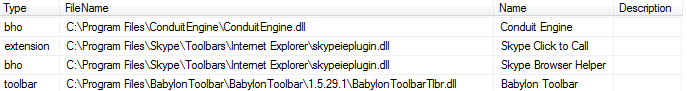
\includegraphics[scale=.8,angle=0]{figures/db_addons_snapshot.png}
\end{small}
\caption{An example SQL table}
\label{fig:db_addons_snapshot}
\end{figure}

The field values correspond to raw information extracted from the users' machines. Accordingly, it lacks normalization. Figure \ref{fig:addons_versioning_snapshot} \textcolor{red}{also here: use examples that include non-empty description values} illustrates the variability across records, which we consider to be co-referent as they describe the same addon. As shown, there are differences across individual records with respect to the path in which the add-on is installed on the local machine, as well as the version number (e.g., 1.8.7.2 vs. 1.8.4.9 in the figure), name and description. Furthermore, the user base is international, and is accordingly multi-lingual.  \textcolor{red}{Say a bit more about the data: is there any add-on attribute that is always populated? path perhaps? how often is the add-on name or description left empty?}
[SELA: Typically in Internet Explorer there is a path attribute, in Mozilla Firefox and Google Chrome browsers there is a name attribute. But in most cases one of the attributes is empty.]

\begin{figure}[t]
\centering
\begin{small}
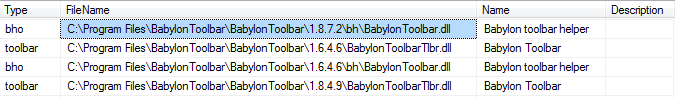
\includegraphics[scale=.8,angle=0]{figures/addons_versioning_snapshot.png}
\end{small}
\caption{An example SQL table with different versions for same addons}
\label{fig:addons_versioning_snapshot}
\end{figure}

Finally, we note another characteristic of interest of this data.  Since the add-ons lists per user are updated on a daily basis, it is straightforward to derive add-on changes (installation and removal) over time. However, there is no tracking of user actions or other programs actions. It is therefore impossible to determine which party initiated any of the status changes; for example, we cannot infer whether a particular addon has been removed (or installed) by the user or automatically, by hostile/protecting program. 

\section{Experimental data}

For the purposes of this study, we consider a subset of the data, including all of the records collected over a  period of two months between Aug. 1 2013--Oct, 1, 2013. Overall, this dataset contains 17,942,715 daily user--add-on associations. It consists of 907,844 unique users and 456,458 unique addons. Figure \ref{fig:user_addons_histogram} shows the distribution of the number of add-ons installed daily per user. As shown,  most users have between 9 and 21 addons installed on their PCs.

\begin{figure}[t]
\centering
\begin{small}
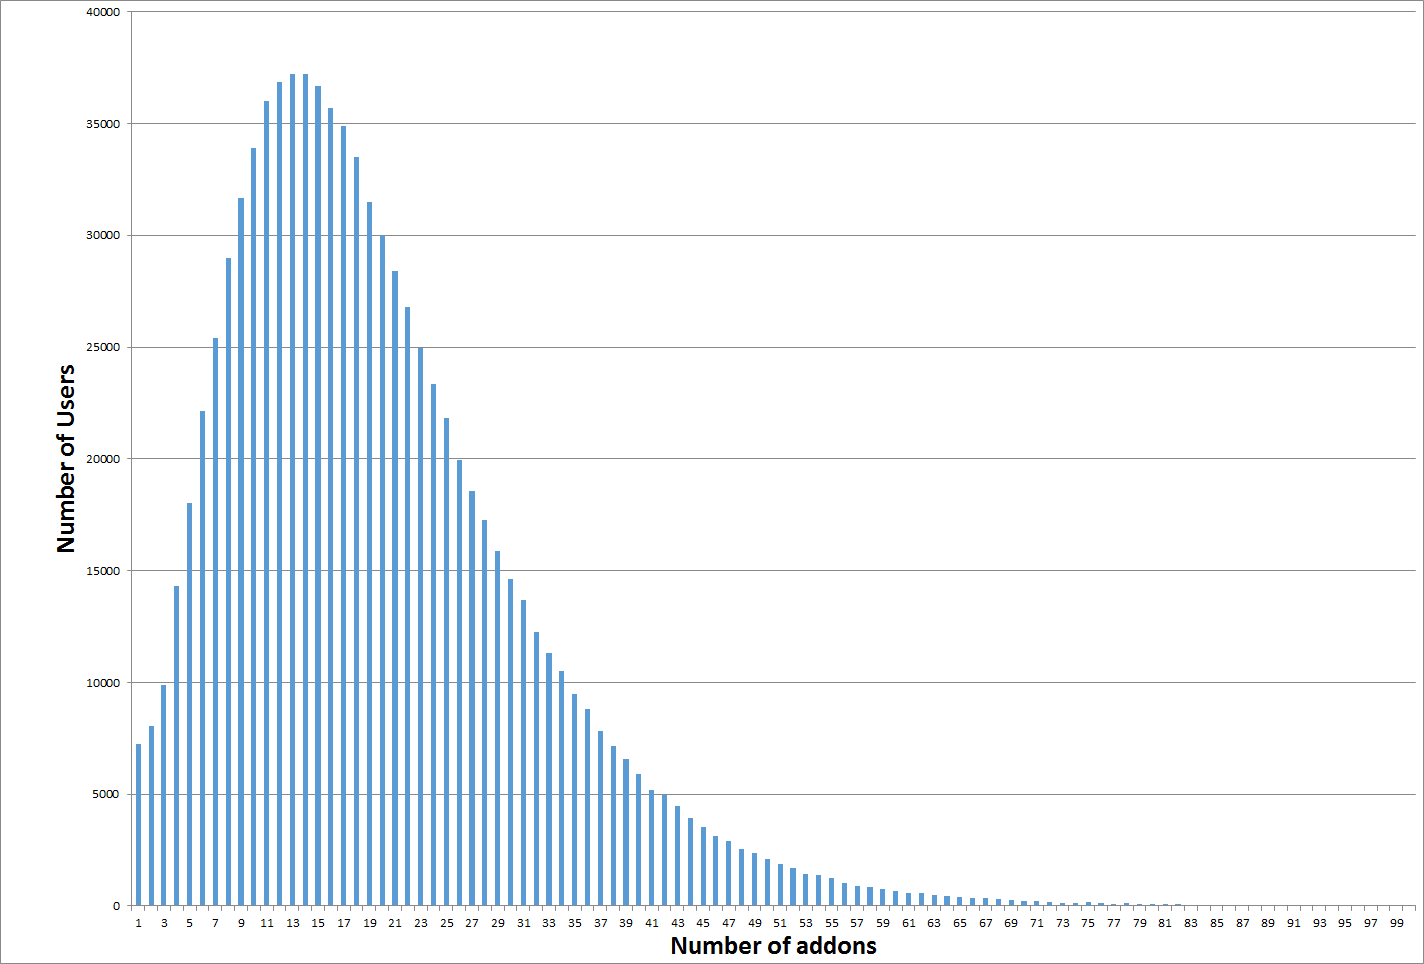
\includegraphics[scale=.9,angle=0]{figures/user_addons_histogram.png}
\end{small}
\caption{Distribution of number of addons per user}
\label{fig:user_addons_histogram}
\end{figure}

In order to enable assessment of textual similarity for record co-reference purposes, we further processed the fields describing each add-on mention into a bag-of-words. These words are represented using {\it terms}, a lexical object type. Given a text string, it is first tokenized, and text cleanup and normalization steps are then applied. For example, we remove non-ASCII characters that serve for encryption purposes on the server. Likewise,  Windows shortcuts for full paths are removed (e.g., VIDEOD$\sim$1 and VIDEOD$\sim$2 and VIDEOD denote the same path), and so forth. Finally, all strings are transformed to lower case, since capitalization is meaningless in this context. Overall, 167,512 unique terms were identified in this process.


\section{Graph representation}

\begin{table}[t]
\begin{center}
\begin{small}
\begin{tabular}{llll}
\hline 
\textbf{source type} & \textbf{edge type} & \textbf{target type} \\
\hline
{\it user} & has-add-on & {\it add-on} \\
\hline
{\it add-on} &  has-add-on$^{-1}$ & {\it user} \\
{\it add-on} & has-term & {\it term} \\
\hline
{\it term} & has-term$^{-1}$ & {\it add-on} \\
\hline
\end{tabular}
\end{small}
\end{center}
\caption{\label{tab:graph_structure} The graph node and directional edge types}
\end{table}

We compactly represent the dataset using a relational graph. Each node in the graph represent a unique, typed,  object.  Concretely, the graph includes the following node types:
\begin{itemize}
\renewcommand{\labelitemi}{$\bullet$} 
\item {\it User} - this node represents user by his unique user id. 
\item {\it Add-on} - this node represents unique addons, where an {\it add-on} is defined as the concatation of all its attributes, namely, file path, addon name and description.
\item {\it Terms} 
\end{itemize}
Directional edges link node pairs.
Table \ref{tab:graph_structure} details the types of edges, representing a variety inter-object relationships, which are derived directly from the relational database structure.
First, we represent the structural relationship between each user and the {\it add-ons} installed on his PC via the {\it has-add-on} edge type, originating at the {\it user} node. An inverse relation exists between each {\it add-on} node and the {\it users} that it is known to be installed at. 
In addition, as described above, each {\it add-on} is associated with its bag of terms representation. Concretely, each {\it add-on} node is linked to {\it terms} contained in either of its attributes over the {\it has-term} relation. Inversely, each {\it term} node is linked to {\it add-ons} that contain it over {\it has-term$^{-1}$} relation.



\iffalse
\begin{small}
\begin{enumerate}[(a)]
\item Go over all users, for each user create a graph node. Graph node name for a user has a prefix "u-" appended to user ID, for example u-00004c1b-8ffc-4ca4-b406-a27e436fa34a node.

\item For each user, go over all its add-ons.
\item For each addon create a graph node, graph node name has a suffix "a-" and appended all addon attributes. For example "a-c:/programfiles(x86)/skype/toolbars/internetexplorer/skypeieplugin.dll"
\item For each addon create term nodes according to its attributes, each term node has prefix "w-" and appedned with a term. For example the addon above would create 6 term nodes:
\end{enumerate}
\end{small}

\begin{itemize}
\renewcommand{\labelitemi}{$\bullet$} 
\item "w-c:"
\item "w-programfiles(x86)"
\item "w-skype"
\item "w-toolbars"
\item "w-internetexplorer"
\item "w-skypeieplugin.dll"
\end{itemize}
%\end{enumerate}
User has edges to all its addons and addon has edges to all it terms, all edges are bi-directional.\\
We have added additional steps for data cleanup.
\fi

\begin{figure}
    \centering 
    \begin{tikzpicture}[
      thick,
      acteur/.style={
        circle,
        fill=black,
        thick,
        inner sep=2pt,
        minimum size=0.2cm
      }
    ] 
      \node (a1) at (5,2.5) [acteur,label=u-00004c1b-8ffc-4ca4-b406-a27e436fa34a]{};
      \node (a2) at (2.5,2.5)[acteur,label=below:a-c:/programfiles(x86)/skype/toolbars/internetexplorer/skypeieplugin.dll]{}; 
      \node (a3) at (-5,0) [acteur,label=below:w-c:]{}; 
      \node (a4) at (-5,1) [acteur,label=w-toolbars]{}; 
      \node (a5) at (-5,2) [acteur,label=w-internetexplorer]{}; 
      \node (a6) at (-5,3) [acteur,label=w-skypeieplugin.dll]{}; 
      \node (a8) at (-5,4) [acteur,label=w-skype]{}; 
      \node (a9) at (-5,5) [acteur,label=w-programfiles(x86)]{}; 
      
      \draw[blue] (a1) -- (a2); 
      \draw[blue] (a2) -- (a3);
      \draw[blue] (a2) -- (a4);
      \draw[blue] (a2) -- (a5);
      \draw[blue] (a2) -- (a6);
      \draw[blue] (a2) -- (a9);
      \draw[blue] (a2) -- (a8);

    \end{tikzpicture} 
    \caption{An example graph view}
    \label{fig:sample_graph}
  \end{figure}
 
  \begin{figure}
    \centering 
    \begin{tikzpicture}[
      thick,
      acteur/.style={
        circle,
        fill=black,
        thick,
        inner sep=2pt,
        minimum size=0.2cm
      }
    ] 
      \node (u1) at (5,4) [acteur,label=u-1]{};
      \node (u2) at (5,0) [acteur,label=u-2]{};
      
      \node (a1) at (2.5,3)[acteur,label=below:a-1]{}; 
      \node (a2) at (2.5,4)[acteur,label=below:a-2]{}; 
      \node (a3) at (2.5,5)[acteur,label=below:a-3]{}; 
      \node (a4) at (2.5,2)[acteur,label=below:a-4]{}; 
 
      \node (w1) at (-3,1) [acteur,label=w-1]{}; 
      \node (w2) at (-3,2) [acteur,label=w-2]{}; 
      \node (w3) at (-3,3) [acteur,label=w-3]{}; 
      \node (w4) at (-3,4) [acteur,label=w-4]{}; 
      \node (w5) at (-3,5) [acteur,label=w-5]{}; 
      \node (w6) at (-3,0) [acteur,label=w-6]{}; 
      
      \draw[blue] (u1) -- (a1); 
      \draw[blue] (u1) -- (a2); 
      \draw[blue] (u1) -- (a3);
      \draw[blue] (u2) -- (a4);
      \draw[blue] (u2) -- (a2);
      
      \draw[blue] (a1) -- (w1);
      \draw[blue] (a1) -- (w2);
      \draw[blue] (a1) -- (w3);
      
      \draw[blue] (a2) -- (w1);
      \draw[blue] (a2) -- (w3);
      \draw[blue] (a2) -- (w4);
      
      \draw[blue] (a3) -- (w1);
      \draw[blue] (a3) -- (w2);
      \draw[blue] (a3) -- (w3);
      \draw[blue] (a3) -- (w4);
      \draw[blue] (a3) -- (w5);
      
      \draw[blue] (a4) -- (w6);
      \draw[blue] (a4) -- (w2);
      

    \end{tikzpicture} 
    \caption{An example graph view 2}
    \label{fig:sample_graph2}
  \end{figure}
  
Figure \ref{fig:sample_graph} \textcolor{red}{It would be good to include another add-on in the figure, or at least, a more interesting add-on, which also inlcudes a name and description} illustrates the graph generation process. Given a user, it is represented by a graph node, where we append the prefix "u-" to the user ID in order to simplfy the identification of node types; for example, in the figure, the user is denoted by the node `u-00004c1b-8ffc-4ca4-b406-a27e436fa34a'. For each user, we iterate over all its add-ons, where each unique add-on is mapped to a graph node. {\it Add-on} graph node names include the prefix "a-", followed by a concatenation of the addon attribute values; in the figure, a single add-on exists, for which only path infomration is availabe, where the respective node name is `a-c:/programfiles(x86)/skype/toolbars/internetexplorer/skypeieplugin.dll'. Finally, each {\it add-on} node is mapped to {\it term} nodes. The term nodes start with the prefix "w-". \textcolor{red}{Did you apply stemming?};, no stemming were applied, for example, the {\it add-on} node in the figure is linked to six term nodes, wich resulted from the string tokenization and processing. 
  
The graph representation of this data has several advantages. Besides being compact, we expect similar entities to reside in high proximity to each other in the graph. For example, the {\it add-ons} named `Skype-US' and `Skype-UK' have non-identical names; however, they share the term `skype', indicating in this case that they are variants of the same add-on. Figure \ref{fig:terms_layer} illustrates how the representation of the full strings results in isolated graph segments, whereas adding the terms nodes yields a connected graph, where the two add-ons are linked over a path that traverses the "Skype" term node.

\begin{figure}[h]
\centering
\begin{subfigure}[b]{0.49\textwidth}
	\centering
	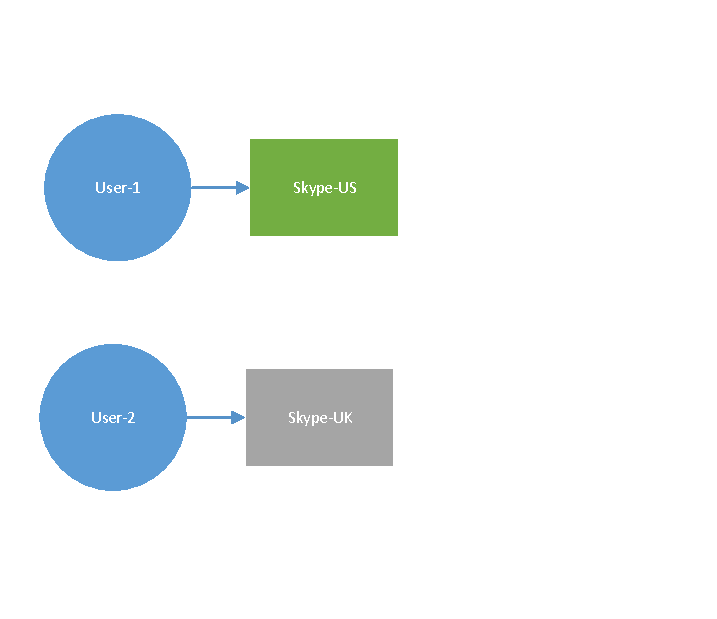
\includegraphics[width=\textwidth]{figures/skype_exampe1.pdf}
	\caption{Without terms layer}
%	\label{fig:skype-no-terms}
\end{subfigure}
\begin{subfigure}[b]{0.49\textwidth}
	\centering
	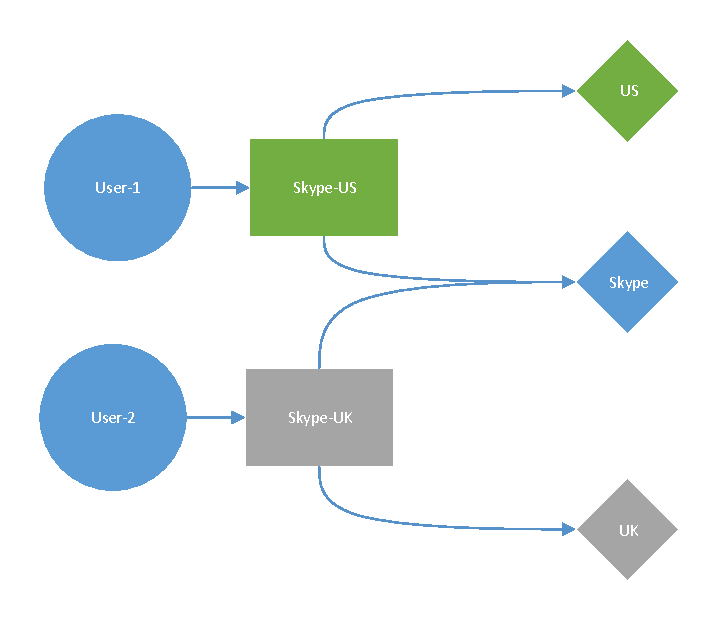
\includegraphics[width=\textwidth]{figures/skype_exampe2.pdf}
	\caption{With terms layer}
%	\label{fig:skype-with-terms}
\end{subfigure}
	\caption{Terms layer example}
	\label{fig:terms_layer}
\end{figure}
  
Figure \ref{fig:sample_graph2} shows another toy graph, demostrating another aspect of inter-user similarity reflected as connectivity patterns in the graph. This gtaph includes two users named shortly as `u-1' and `u-2'. The two users are similar in that they share two add-ons, `a-1' and `a-2'. In addition, while {\it add-ons} `a-3' and `a-4' are distinct from each other, these add-on nodes are connected via the common term node `w-2'. 

We will apply random walks in the graph in order to assess similarity, or relatedness, between users and add-ons.  

\subsection{Data statistics}

The experimental dataset corresponds to a graph that consists of 1,331,814 nodes and 18,552,622
edges. \textcolor{red}{Detail the number of nodes by type in a table}. 

\begin{figure}[t]
\centering
\begin{subfigure}[b]{0.49\textwidth}
	\centering
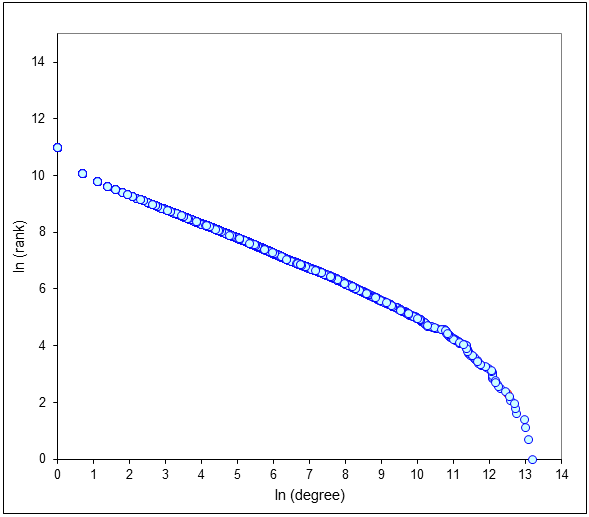
\includegraphics[scale=0.49]{figures/zipf_addon.png} \\
\caption{add-ons} 
%\label{fig:minlen2noremoveRecall}
\end{subfigure}
\begin{subfigure}[b]{0.49\textwidth}
	\centering
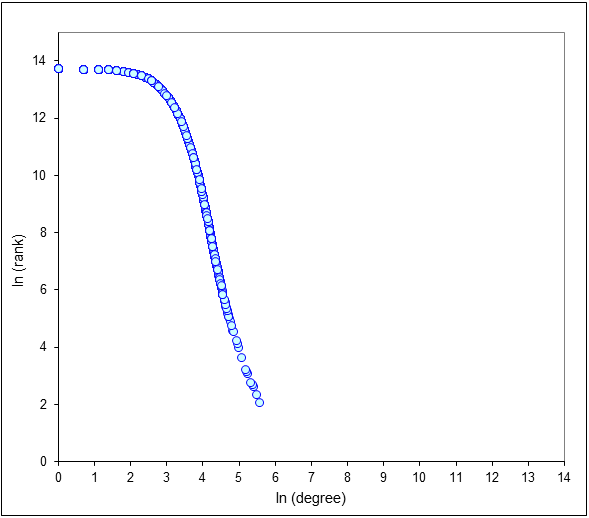
\includegraphics[scale=0.49]{figures/zipf-users.png} \\
\caption{users}
%\label{fig:minlen2noremoveMRR}
\end{subfigure}
	\centering
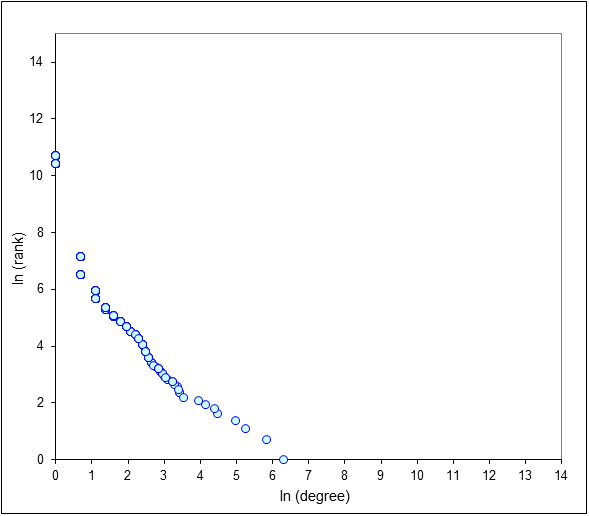
\includegraphics[scale=0.48]{figures/zipf-terms.png} \\
(c) terms \\
\caption{Log-scale rank vs. degree plots of add-ons (a), users (b), and terms (c)}
	\label{fig:minlen2noremove}
\end{figure}

\chapter{The missing addon in User ecosystem}
\label{fig:zipf}
\iffalse
\textcolor{green}{\textit{Einat: Start by introducing the problem, why it is interesting..}}\\
\fi

As described in the previous chapter, we consider authentic user-addon
associations represented as a graph.  The graph includes typed nodes
denoting {\it user}, {\it addon} and {\it term} entities. Structured
relations, between {\it users} and the {\it addons} that exist on
their machines, are represented by bi-directional graph edges. We
treat the graph as a sample of the add-ons eco-system. Thus, we expect
to observe phenomena such as species (add-on) co-existance patterns in
this eco-system; supposedely, complimentary add-ons, or add-ons
installed by ally parties, will be found in the same machines;
likewise, rivlary species will not co-exist in the same environments
(machines).

In this chapter, our focus is on alliances that underlie add-on
distributions, manifested as postive correlations between add-ons
installed on the users' machines. Concretely, we are interesting in
addressing the following question:

{\it Given partial information about the population of add-ons that
  exist the machine of an individual user--how sussccesully can we
  infer the identity of additional species (add-ons) that exist in
  that environment?}

If we can indeed predict with high certainty missing members in a
local community, then this should verify the existance, as well as
indicate the strength of such correlations. The merit of the stated
question is that it can be readily evaluated empirically. We report a
set of experiments, where the link between a random {\it user} and one
of the {\it add-ons} associated with this user is artificially
removed. The task then becomes an instantiation of the {\it link
  prediction} problem, where the goal is to reveal a new association
of interest ({\it has-add-on}, in this case) between graph nodes.

Link prediction is odten manifested in terms of semantic similarity,
where there exist numerous graph-based similarity measures that may be
readily utilized for this purpose. We use in this work Personalized
PageRank (PPR), a random walk based similarity metric in graphs.

Below, we first formulize the task, and describe how PPR is used to
tackle this task. We then turn to describing our experimental dataset
and setup, and discuss our results. This chapter ends with a
discussion of our main findings.


\section{Task definition}
\label{sec:task}

Let us denote the graph nodes $G$ as a union of $U,A,T$, the sets of
{\it users}, {\it add-ons} and {\it terms}, respectively. We view this
graph as a global ecosystem. An individual user $u\in U$ is linked in
the graph to its set of add-ons $A_i$. Let us remove a single item $a$
from $A_i$. User $u$ would be then associated with the modified {\it
  add-on} set $A'=(A-A_i)$. Our goal is then to predict the identify
of {\it add-on} $a$ that has been removed, thus predicting the missing
link between $u$ and $a$.

In the rest of this chapter, we will usually refer to the set $A'$ as
a {\it query}. As in information retrieval, our goal would be to
assess the relrevancy of possible responses to the
query. Specifically, the candidate responses in this case are the
known {\it add-ons}, which are not known to be associated with the
user, i.e., $(A-A')$, where this candidate set includes $a$. As
described below, we use a ranking approach, where the candidate {\it
  add-ons} are ranked by their estimated relatedness to the user node
$u$. It is important to note that the rankings are specific to the
dynamic queries, reflecting the estimated relevancy with respect to
the query.

[EINAT:]AN ISSUE: There are several aspects of this problem. Correlations may
be due to user's tastes, especially for users who are actively
involved in the maintancne of their machine. Another factor is
functionality, where we may expect to find complimentary
add-ons. Finally, there may be positive correlations due to
manipulations in the automatic installations, reflecting business
alliances. A limitation of this study is that we have no evidence
whatsoever about the specific factors that led some add-on to be
installed on one's machine. WE DO NOT MODEL THESE FACTORS
SEPARATELY. Perhaps say that these different types of co-existance are
also exhibited in biological eco-systems?

\section{Approach}
\label{sec:method}

We employ a well-studied graph ranking algorithm, Personalized
PageRank \citep{page1999pagerank}, to compute query-specific relevancy
scores based on the link structure of the graph. In this paper, we use
the rankings of Personalized PageRank, as a criteria for recommending
an addon. Taking a specific set of user addons as PPR input query, a
ranking over all the other addon nodes can be leveraged for the
detection of missing addon in user ecosystem.\\

\subsection{Personalized PageRank}
\label{sec:PPR_addons_method}

The well-known (non-personalized) PageRank algorithm measures the
relative importance of web pages, as reflected by their centrality in
the graph structure of the Web \citep{page1999pagerank}. The algorithm
models the bahavior of a random surfer, who at any given time, chooses
between two possible actions: following a hyperlink on the current
Webpage to a related Webpage, or ``re-setting'', jumping randomly to
one of the pages on the Web. Formally, the distribution over the graph
nodes at time $d$ can be computed iteratively, as follows:
\begin{equation}
V_{d+1} = (1-\alpha) [{1 \over N}]_{1 \times N} + \alpha \transition V_d
\label{eq:pagerank}
\end{equation}
\iffalse
\[
\transition = dL + (1-d)[{1 \over N}]_{N \times N}
\]
\fi where the total number of nodes (pages) is $N$, and $\transition$
is a transition matrix, modeling the probability that the surfer moves
to page $j$ from page $i$ following a hyperlink. The probability that
the surfer chooses to follow some hyperlink is $\alpha$, and the
probability of re-setting the walk is ($1-\alpha$) .

\iffalse
$\transition$ distributes a node's probability uniformly among the pages it links
to, i.e.
\begin{equation}
\transition_{ij} = \left\{
\begin{array}{lll}
{1 \over |ch(i)|} & \mbox{if there is an edge from $i$ to $j$} \\ 0 &
\mbox{otherwise}
\end{array}
\right.
\label{pagerank_edge_weights}
\end{equation}
where $ch(i)$ is the set of nodes that have an outgoing link from $i$
(the children of $i$).
\fi 

Due to the reset operation, the random walk process is guaranteed to
converge to a unique stationary distribution $V^*$ (i.e., $V_d$
converges to $V^*$). The {\it PageRank score} of node $j$, $p_j$, is
defined as its probability in the stationary state $V^*$, giving a
measure of document centrality in the network. In general, a node is
assigned a high PageRank score if the sum of the ranks of its
backlinks is high, that is, if it is linked to by other important
Webpages.


The PageRank algorithm described computes universal node importance,
or `centrality' scores, soley based on the network structure, that is,
ignoring user preferences. The {\it Personalized PageRank} variant
\cite{pagerank,RichardsonNIPS02} biases the random walk model to
generate rankings that reflect user preferences, represented as a
distribution of interest over the graph nodes. This bias is modeled by
a small and natural adaptation of the PageRank random walk
formula--instead of assuming that the user is equally interested in,
and would reset to, any graph node uniformly, it is assumed that only
a subset of the graph nodes are of interest to the user, and the reset
operation is accordingly directed to those nodes . The enhanced random
walk scheme is defined as follows:
\begin{equation}
V_{d+1} = (1-\alpha) V_u + \alpha \transition V_d
\label{eq:ppr}
\end{equation}
where $V_u$ denotes a distribution of interest over the graph nodes,
e.g., nodes that are known to be of interest to user $u$.  The
Personalized PageRank scores are derived from the corresponding
stationary state distribution. 

The generated Personalized PageRank scores reflect structural
similarity, or relevancy, of the graph nodes with respect to the
query. It has been shown that the Personalized PageRank score for a
target node $z$ and a query node $x$ equals a summation over all of
the connecting paths between $x$ and $z$ (including cyclic paths, and
paths that cross $z$ multiple times), where paths are weighted by
their probability \cite{jehWWW03,fogaras05}. In words, the graph walk
distributes probability mass from a start distribution over nodes
through edges in the graph---incidentally accumulating evidence of
similarity over multiple connecting paths. Due to the reset
probability $(1- \alpha)$, the paths between $x$ and a destination
node $z$ are weighted exponentially lower as their length
increases. This implies that graph nodes that are connected to the
query nodes over shorter connecting paths, as well as over multiple
connecting paths, are considered more important.

Computationally, the genration of PPR scores is expensive compared
with PageRank scores, since node relevancy is evaluated with respect
to a given query. Fortunately, the computation for a multi-node query
is no more difficult than for a single-node query due to the
\textit{Linearity Theorem} \citep{jeh2003scaling}, as the Personalized
PageRank vector for a multi-node query is a simple linear combination
of the individual PPV for each node in the query.

\iffalse
The graph walk process (and accordingly, the similarity measure
generated) is determined by the graph's topology.\footnote{The reset
probability $\gamma$ has negligible effect on the generated rankings;
see a related discussion in Section \ref{sec:graph_walk_parameters}.}
In addition, the walk on the graph is controlled by a set of edge
weight parameters $\Theta$. This means that throughout the graph,
edges of type $\ell$ are assigned a typical edge weight $\theta_{\ell}
\in \Theta$. Let $L_{xy}$ denote the set of edge types of the outgoing
edges from $x$ to $y$. The probability of reaching node $y$ from node
$x$ over a single time step (corresponding to the transition
probability $\transition_{x,y}$) is defined as:

\begin{equation}
Pr(\edge{x}{}{y}) = 
{\sum_{\ell \in L_{xy}}\theta_{\ell} 
\over 
\sum_{y' \in ch(x)}\sum_{\ell' \in L_{xy'}}\theta_{\ell'}}
\label{eq:transition1}
\end{equation} 
where $ch(x)$ denotes the set of children of $x$ (the nodes reachable
from $x$ in one time step). That is, the probability of reaching node
$y$ from $x$ is defined as the proportion of total edge weights from
$x$ to $y$ out of the total outgoing weight from the parent
$x$.\footnote{The PageRank scheme given in Formula
  \ref{pagerank_edge_weights} is a special case of Equation
  \ref{eq:transition1}, where the graph includes a single edge type,
  and weights are distributed uniformly.} The graph edge weights
$\Theta$ can be set uniformly; randomly; manually, according to prior
beliefs; or using a learning procedure. The edge weights $\Theta$
provide another mechanism for affecting the probability flow in the
graph.
\fi

As mentioned before, the algorithms of PageRank and Personalized
PageRank algorithm have been designed so as to improve Web page
rankings. The Personalized Pagerank variant was first suggested in
\citep{brin1998can}, and shortly after, has been explored to
personalize Web search
(\citep{haveliwala2002topic},\citep{haveliwala2003topic},\citep{haveliwala2003analytical}). Nevertheless,
PageRank may be readily applied to arbitrary graphs to produce node
importance scores, and this places PageRank amongst a class of network
analysis techniques \citep{brandes2005network} known as centrality
measures or indices \citep{koschutzki2005centrality}. Similarly,
Personalized PageRank is a general similarity measure in graphs, used
in multiple domains. For example, iIn \citep{freschi2007protein}, the
authors used the Personalized PageRank model, which they call
ProteinRank, to predict protein functions.

\iffalse In this thesis the goal of biasing the PageRank with the
teleportation vector is to personalize the user addons of choice
results.  Instead of looking at a “random surfer” on the web, the
non-web PageRank models a random walk on the graph. The behavior of
the walk is the same as the random surfer: with probability $\alpha$
the walk continues along an edge of the graph and with probability
1-$\alpha$ the walk jumps to a random node in the graph. Personalized
PageRank is an important extension of PageRank model, in which the
surfer does not randomly restart browsing anywhere on the web after
choosing not to follow a link. Rather, the surfer in this new model
restarts at one of only a few pages. If the pages relate to one
person, then the resulting PageRank vector is called a personalized
PageRank vector. If the pages are topically related, then the vector
may be called a topic-specific PageRank vector.  \fi

\iffalse
Personalized PageRank is an extension of the famous PageRank algorithm
\cite{page1999pagerank}, both of which are based on a random surfer
model. To understand Personalized PageRank, we first review the
original PageRank briefly. A random surfer starts at any node on the
graph. At each step, with a probability of 1−$\alpha$ the surfer moves
to a neighboring node randomly, and with a probability of $\alpha$ he
teleports to a random node on the graph. This process is repeated
until the walk converges to a steady-state. The stationary probability
of the surfer at each node is taken as the score of the node. However,
this form of score is purely based on the static link structure,
indicating the overall popularity of each node on the graph, without
tailoring to a specific query node.\\ In contrast, Personalized
PageRank enables query-sensitive ranking, in the sense that we can
specify a query node to obtain a “personalized” ranking
accordingly. It is based on the same random surfer model of the
original PageRank, except when the surfer teleports, he always prefers
the query node \textit{q}. Specifically, at each step, with
probability $\alpha$ the surfer teleports to \textit{q} instead of a
random node, thus visiting the neighborhood of \textit{q} more
frequently.  Thus, the stationary distribution, called a Personalized
PageRank Vector (PPV), is biased towards \textit{q} and its
neighborhood, which can be interpreted as a popularity or relevance
metric specific to \textit{q}.  More generally, a query \textit{q} can
comprise multiple nodes on the graph, such that in the teleportation
the surfer can jump to any node in \textit{q}. Fortunately, the
computation for a multi-node query is no more difficult than for a
single-node query due to the \textit{Linearity Theorem}
\citep{jeh2003scaling}, as the PPV a multi-node query is a simple
linear combination of the individual PPV each node in the query.

A personalized PageRank vector, also known as a random-walk with
restart (RWR), is the stationary distribution of a random walk that,
with probability $\alpha$ follows a step of a random walk and with
probability (1−$\alpha$) jumps back to a seed node.  If there are
multiple seed nodes, then the choice is usually uniformly random. The
set of these seeds is called personalized PageRank Vector (PPV).  
\fi

In this thesis, we apply the Personalized PageRank model to our graph
repreesnting the add-oneco-system, as described in detail in the next
section. 

\iffalse 
with users and looking for their personal
preferences in browsers extensions, we are also interested in Company
based addons propagation in users network. All our dataset was
transformed to undirected graph, where user nodes are connected to
addon nodes according to their relationship in the original dataset,
e.g. each user node has an edge connected to addon node if this user
has this addon installed in its ecosystem. Since our goal is to
determine/predict a missing addon in user ecosystem, the seed nodes
for the personalization vector would be the specific user addons, our
hypothesis is that a higher the PageRank score suggests a higher
relevance of an addon to the specific user. We would run multiple
experiments to show the correctness of our hypothesis.  
\fi

\iffalse
\subsection{Support Vector machine}
First we have tried running analysis on our data using SVM. We were
trying to classify users that are staying long in user ecosystem and
those that churn immediately, lately this would turn to Clash
prediction.\\ We have defined training data as follows - positive
examples are the users that have stayed at the system more than three
days and others are negative example. We have used a popular libSVM
tool to run the analysis.\\ The training very long time and gave no
results, trying to run SVM with another kernel did not help either -
and every run took a few days to finish. Then we've decided to find
another way to represent our data.
\subsection{GraphChi}
\subsection{iGraph}
\fi

\subsection{Applying PPR to find the missing add-on}

We address the task of add-on list completion in terms of structural
similarity in the graph. The question that we wish to answer is `given
a set of {\it add-ons}, which are known to co-exist on the machine of
some user, what other {\it add-ons} are most likely to be linked to
that user?'. This question is addressed by means of structural
similarity in the graph.

Formally, we assign $V_u$ to be uniform over $A'$, that is, the re-set
probability to each of the nodes representing {\it add-on} $a\in A'$
is set to ${1 \over \mid A' \mid}$, and is zero otherwise.

The transition matrix $\transition$ assign equal importance to all of
the graph edges. In words, the transition probability from node $i$ to
a linked node $j$ is defined as: $_{ij}={1 \over \mid N_i \mid}$,
where $N_i$ is the set of nodes linked over an outgoing edge from $i$,
i.e., the {\it outdegree} of node $i$. For example, suppose that node
$i$ is linked to two {\it term} nodes and five {\it user} nodes; then,
the probability of reaching any of these nodes using the transition
operation equals ${1\over 7}$. As the transition probability are
  directly derived based on outgegree, the notion of {\it inverse
    document frequency} is implicitly modeled in the transition
  model. In particular, nodes that are linked to a large number of
  other nodes will pass only a fraction of their probability mass to
  connected nodes; indeed, highly frequent entities (e.g., the {\it
    term} `version'), for which the inverse frequency is low, are less
  meaningful. In contrast, nodes linked to a limited number of
  neighbors, carry high information value. 

In general, it is possible to assign different edge weights according
to edge types. Recent works have also considered learning a selective
set of meaningful paths in the graph that link query with target
nodes. We leave the exploration of these methods of supervised tuning,
given labeled examples, to future work. 

The computed Personalized Pagerank vector assigns scores to all of the
graph nodes. We consider the graph nodes of type {\it add-on} and rank
them by their score. It is conjectured that the `missing add-on' will
be included among the top-ranked items in the list, due to high
structural coherence with the input set of add-ons observed in the
user's environment.

More concretely, we expect relatedness to flow over multiple path
types, reflecting various types of structural similarity in the graph,
mainly:
\begin{itemize}
\item {\it co-occurrence patterns}: A dominant, short, path that
  directly leads to related add-ons is {\it add-on} $\Rightarrow$ {\it user}
   $\Rightarrow$ {\it add-on}; this path links a node denoting an input add-on
  with other users that have that add-on installed on their
  machine. Walking from these {\it user} nodes to their associated
  {\it add-ons} should highly weight those add-ons that frequently
  co-occur with the input add-on. As the query consists of multiple
  {\it add-on} nodes, the result of the random walk process is the
  aggregated score vectors, meaning that other add-ons, which co-exist
  on users' machines with multiple input add-ons will be prioritized
  in the rankings. 
\item {\it term-based similarity}: As demonstrated before
  (Sec. \textcolor{red}{x}), the name and descriptions of add-on
  instances are varied. In particular, the same add-on may include
  different version numbers. The representation graph links each {\it
    add-on} node with the {\it terms} that it contains. Thus,
  co-reference can readily take place via the path {\it add-on}
  $\Rightarrow$ {\it term} $\Rightarrow$ {\it add-on}. Also here,
  probability mass is mainly propagrated over this path between {\it
    add-ons} that share multiple {\it terms}.
\end{itemize}

To the extent that the random walk process is applied until its
convergence point, long-range relationships in the graph are
manifested in the stationary distribution, consisting in this case
also of the concatantaion of the short paths listed. In this fashion,
we expect that co-occurrence of coreferent items will be also
reflected in the random walk results.

PLACE IN RELATED WORK: In Keren's thesis, we have shown that PPR's
random walk similarity metric outperforms classical collaborative
filtering and content-based recommendation methods.


\section{Experimental methodology}

Given the collected corpus, we derive sets of labeled queries for evaluation purposes.  Each query corresponds to a randomly selected user $u$. We randomly select one of the user's add-ons, $a$, and eliminate it artificially from the user's `profile', having the link between the nodes denoting $u$ and $a$ disconnected in the graph. In
the experiments, we evaluate the extent to which the missing link can
be recovered. 

The process of generating an individual labeled example is formally outlined in Figure
\ref{fig:example-gen}. Naturally, the sampled users are required to have at least two addons installed on their machine--otherwise, the query vector would be left empty, once removing the add-on from the user node for testing purposes. 

\begin{figure}
\begin{enumerate}[(a)]
\begin{small}
\item Pick uniformly at random a {\it user} node $u$ from the graph.
\item Find the set of {\it add-on} nodes linked to $u$, $A_u$.
  all its addon nodes.
\item Pick uniformly at random an addon node $a$ from the set $A_u$. 
\item Disconnect the link between nodes $a$ and $u$ in the
  graph. Since the only connection between a user node and the addon
  node is the edge between them, by simply deleting this edge we are
  removing this addon from user profile.
\item Let the query $V_u$ be a uniform distribution over $\{A_u-a\}$,
  and the correct answer to the query be $a$. 
\end{small}
\end{enumerate}
\caption{The process of generating an individual labeled example}
\label{fig:example-gen}
\end{figure}

The labeled examples thus consist of queries, which include the addons still associated with {\it user} $u$, and a single known correct response, which is the removed addon $a$.
Once disconnected from the user node, there should be no selection bias towards the target add-on $a$ compared with the other 200 thousand addon nodes. Assuming that addons are mutually related, the ranking scheme should identify strong association between the removed add-on and the environment of remaining add-ons associated with the same user. Accordingly, we expect to find the missing add-on among the top ranks of the list with high probability. Obviously, the add-ons already associated with the query user are  typically assigned high relevancy scores by query-sensitive algorithms like PPR. Importantly, we remove the query add-ons from the evaluated ranked list. 

\subsection{Evaluation measures}

\iffalse Now, like in \autoref{sec:PPR_addons_method},
when we are predicting the missing add-on, we are looking at the
addons ranking list (the ranking is according to PageRank scores) and
check the Recall@K. This measure seems to give similar results as the
Popularity baseline.\fi

All of the evaluated methods produce a ranked list of add-ons. 
Concretely, the PPR and PageRank algorithms compute scores for all of the graph nodes.
It is straight-forward to filter the nodes by their type, and output a ranked list that consists of add-ons only.


\iffalse Since, lets say it is ranked in 8th position, not
taking into account the ranking position of the original user addons,
then we could recommend to user top ten scored addons and with high
probability user will find a usefull addon between this
ten.\\ \textcolor{green}{\textit{Sela: Example:}}
\textcolor{green}{\textit{Einat:How was evaluation conducted? cross
    validation.. using MAP meausre(?)  (can include a description of
    MAP as an appendix)}} \fi

We use a set of standard information retrieval metrics for the evaluation of the output ranked lists. Note that in our settings, there is a single `correct' answer. The various metrics assess the quality of each algorithm by the extent to which it succeeds to 
place the relevant node at high ranks on average, across all queries. A short description of the evaluation measures follows.

\paragraph{Recall at k (Recall@k)}
This is the fraction of queries, for which the relevant response is included among the top $k$ ranks, as formulizaed in Eq.~\eqref{eq:rec-at-k}. \textcolor{red}{Sela: the equation need to be modified: first, it is the average scores acorss multiple queries. Lets assume that we have $N$ queries. Second, account for the fact that we have a single correct response per query. You use a general definition of recall, but you should really used a formula for recal-at-k}. This criterion captures the quality of rankings for applications where the first few results matte most. 
For recommendation systems, users usually will only view several top ranked candidates. Therefore
whether the correct addon exists in the top ranked candidates is
important, and Recall@k is designed for measuring this. \textcolor{red}{Need to discuss how to introduce the missing add-on problem alongside a recommendation application.}
\begin{equation}
 Recall = \frac{number \, of \, relevant \, documents \, retrieved}{number \, of \, relevant \, documents}
\label{eq:rec-at-k}
\end{equation}
\iffalse
\begin{displaymath}
 Precision = \frac{number \, of \, relevant \, documents \, retrieved}{number \, of \, retrieved \, documents}
\end{displaymath}
\fi


\paragraph{Mean Reciprocal Rank (MRR)}

The mean reciprocal rank \citep{voorhees1999trec} is a
well-known evaluation metric in Information Retrieval (IR), which considers the position of the first correct
answer in the ranked list.  As formulized in Eq.~\eqref{eq:mrr}, the reciprocal rank is the inverse of the position of the first correct addon in the ranked set of addons produced for a given query; the MRR is the average of the reciprocal ranks across all of the queries. Unlike the recall@k measure, which disregards the results below rank $k$ for evaluation purposes, MRR consider the full list of ranked items. It is especially informative in assessing recommendation quality in domains that target a small set of valuable items \citep{chen2006less}, such as friends recommendation in social
networks. In our settings, there is a single correct answer per query. It is desired to include the missing add-on, and possible other relevant add-ons that can be recommended to the user, at high positions of the ranked list.
\begin{equation}
 MRR = \frac{1}{Q} \times \displaystyle\sum\limits_{q=1}^{Q} \frac{1}{rank(1^{st} \, relevant \, result \, of \, query \, q)}
\label{eq:mrr}
\end{equation}

\subsection{Statistical validity}

Overall, we generated datasets that include $N=1000$ labeled examples, each sampled from a unique user...

\textcolor{red}{Give a detailed example of a query?}
Explain that the 1000 were chosen uniformally at random
also explainx4k
\textcolor{red}{What else can we say here?.. are the selected users in
  the dataset and corpus multi-national, or geographically focused?
  any other characteristics worth mentioning?}

\iffalse
\textcolor{green}{\textit{Einat:Used Personalized PageRank -- which parameters? how were the paramater
values set?}}
\fi


\section{Experiments}
\label{sec:experiments}

We use Personalized PageRank to rank {\it add-on} nodes in
the graph by their structural similarity to the user profile, or {\it
  query}. The generated rankings using this approach may be affected
by design choices concerning the graph structure and the random walk scheme. This section first provides details regarding the implementation of PPR, as well as baseline methods that we compare against. It then discusses several aspects concerning the graph design that are evaluated in this work.

\subsection{Methods}
\label{sec:methods}

\subsubsection{PPR} In this research, we experiment with a fast and memory-efficient implementation of Personalized PageRank included in {\it igraph} \citep{igraph}, a software library optimized for the processing large-scale graphs. {\it iGraph} uses internally the ARPACK package, a numerical software library written in FORTRAN 77, for solving large
scale eigenvalue problems (used also in Mining and Analyzing Social
Networks book \textcolor{red}{?--cite}). Concretely, ARPACK applies an implicitly restarted Arnoldi method to calculate the random walk scores. \iffalse igraph expects as an adjacency list of numeric
vertices. We have created a unique number for each node and store the
mapping to an actual node name in a separate file.\fi The computation of PPR scores is highly efficient, as the whole graph is loaded into memory. \iffalse, we had to be very careful with memory
management (every very small leak would cause a serious global memory
leak).\fi We ran the experiment using a standard PC machine with x memory using a a 64bit version of igraph. On average, running a batch of 1,000 queries required only x--y seconds. In the experiments, we set the teleport probability parameter $\alpha$=0.85 following previous works. In general, due to the exponential decay over distance from the query nodes implied by PPR's random walk formula, the teleport probability values has negligible effect on the produced rankings.


We compare our algorithms against two strong baselines: ranking {\it add-ons} by `popularity', as well as based on their PageRank scores. 

\subsubsection{Popularity baseline} 
A simple approach for predicting the `missing' add-on would be to rank the {\it add-on} items by their popularity, determined by the total number of users associated with each add-on in the dataset. Using this approach, the response to all queries is equal and fixed, having the output list ranked according to the popularity criterion. In other words, since the algorithm performs no personalization, all users are presented with the same
add-on list. Despite its simplicity, the popularity algorithm can perform reasonably well when item popularity follows a power law distribution  \textcolor{red}{cite Keren's thesis}. Another advantage of this algorithm is that it is non-parametric and scalable; item scores may thus be computed efficiently for datasets containing hundreds of thousands of users and tens of millions of items by means of database querying. 

\subsubsection{PageRank baseline} 
For each addon we have calculated its PageRank score given the underlying graph. The PageRank scores assigned to the graph nodes 
reflect their structural centrality in the graph. We are interested in comparing PPR performance with this non-personalized version of the random walk algorithm.

Both baselines were implemented using {\it igraph}. \iffalse were implemented in a high performance, parallel
or distributed environment. We chose to use igraph \citep{igraph}, a
high-performance, parallel machine learning framework. \fi

\subsection{Graph design choices}
\label{design}

The proposed graph schema is simple and natural in the sense that it directly represents the relational structure of its source information. We discuss in this section a set of considerations involved in fine tuning of the graph design. The impact of the design options detailed below is evaluated empirically.  

\subsubsection{Pruning of high-degree nodes} 

Several previous works have indicated that high-degree nodes in the graph have negative impact on the PPR similarity measure (\textcolor{red}{cite the Pizzaman work}). First, high density of the transition matrix results in increased computation cost of the random walk process. Further, the random walk process exhibits some bias in favor of high degree nodes. Removing such high degree nodes should only result in only a small approximation error [cite Purnamrita Sarkar], while improving performance by increasing the `visibility' of lower-degree
nodes. Following previous works \textcolor{red}{can we cite any?},
we experiment with a graph variant, in which high-degree nodes are
removed. We set the threshold over a node's out-degree to 500 in this
work. As shown in Figure~\ref{fig:zipf}, only a fraction of the most popular {\it add-ons} have a greater out-degree and are pruned in this fashion. Note that given a graph variant in which these `popular' nodes have been removed, the sampled queries include {\it add-ons} that may be less trivial to predict. One may find special interest in this configuration for the purpose of recommending {\it add-ons} as the recommendation of highly popular and possibly familiar {\it add-ons} may be less beneficial for some users. 

\subsubsection{Specificity of path information} 

Add-on names often include full file-system path information, e.g., `C:/Program Files (x86)/...'. We remove path prefixes (like `C://Program Files (x86)') in our main experiments for several reasons. First, we wish to represent every unique add-on as a distinct node in the graph. Including path details in the add-on name will result in multiple copies of the same add-on merely due to differences in local installation sites. Such redundancy may have negative effect on the produced  graph-based node relatedness metric, as well as bias the evaluation. Suppose that the target add-on is included in the answer list with a path prefix that is different from the one used in the target user's machine; if we kept the path, then it would be considered as incorrect answer, while removing the path should help us to identify it as the same add-on. In addition, Supposedly, it can be harmful to link add-ons to common {\it terms} associated with path information (e.g., `program'; `files'; `x86'). Such links may connect add-ons due to machine configurations that are meaningless semantically.

\subsubsection{Term modeling}

The modeling of {\it term} nodes is desirable as it establishes links between related addons, e.g., add-ons with the same name but with different version numbers. Specifically, version numbers are included either as a suffix to the add-on name, or as a directory name part of the path string. Splitting the add-on names into tokens and linking the respective {\it add-on} and {\it term} nodes should maintain connectivity between multiple version of the same {\it add-on}, where consequently this should improve the graph relatedness measure. \textcolor{red}{does this help also when the version number is in the suffix?} On the other hand, it is possible that linking {\it add-ons} over shared {\it terms} will result in a topical drift. Assuming, for example, that the user is known to have an {\it add-on} that has to do with video streaming and has the term `video' as part of its name; other {\it add-ons} reached by traversing a term-hopping path may have similar functionality. In this fashion, given the user's query, the ranked list of results may include {\it add-ons} that are similar or alternative to the {\it add-ons} that are known to be installed at the target user, pushing downwards in the rankings those {\it add-ons} that are complimentary to the user\s eco-system. Experimental results using graphs with and without {\it term} nodes shows that overall, term modeling has positive effect in predicting the `missing' add-on.

\section{Results}

\iffalse
1) `default' scenario:

Use the graph with popular nodes. Compare these variants:
- Popularity baseline
- PageRank baseline
- PPR, users+addons, without paths
- PPR, users+addons+terms, without paths

Show results for 4X1000. MMR / recall@k.

Main findings: we outperform popularity; also, representation of terms helps.

2) Focus on lower-degree add-ons:

- The scores are approximately correct when high-degree nodes are removed.
- Reduces computational costs.
- Low-degree nodes are interesting, but popularity and PR methods only include them at the bottom of the list.

2A) Include analysis of degree distribution: 
-- show number of nodes by degree, log-scale. (look for example graphs of Zipf's law).
-- Same, for add-ons.
-- Same, for terms.
-- Same, for users. (do not use log-scale if it doesn't make sense, as in this case.)

2B) Use the graph without high-degree nodes. (Re-compute the pop. and PR baselines.)
- Popularity baseline
- PageRank baseline
- PPR, users+addons, without paths
- PPR, users+addons+terms, without paths

SENSITIVITY:

3) Impact of paths:

What happens if we include the full path?

Detail number of add-ons before and after filtering. 

- Full graph, users+addons+terms
- High-degree removed, users+addons+terms

- Full graph, users+addons
- High-degree removed, users+addons

4) Sensitivity to # of add-ons per user: (>=2, >=3, ..)

Can show results of multiple configurations as curves on the same graph.
\fi

Our main goal in the experiments is to assess the extent to which add-ons co-exist in one's environment. Extensive experiments were conducted, optimizing system design so as to obtain an effective and valid structured similarity metric. In this section, we report the evaluation results of the different components of the system, as well as compare it against viable baselines.  

\paragraph{Main results}

We report experimental results method.For each of the methods we report Recall@10, Recall@50,
Recall@100 and MRR as described at \autoref{sec:ranking}. 


As shown in \autoref{fig:minlen2remove500Recall}, our algorithm has correctly
predicted a missing addon at top-10 ranking list addons, in
{$\sim$}42\% cases. \textcolor{red}{Are these average results of multiple runs, or just of 1000 queries batch?} It is also greatly outperforms the baseline
benchmark. We have also compared the Mean Reciprocal Rank (MRR) of our
algorithm and the baseline as shown in
\autoref{fig:minlen2remove500MRR}. \textcolor{red}{Add baselines to the figure; discuss in detail.}

\begin{figure}[h]
\centering
%\begin{subfigure}[b]{0.49\textwidth}
	\centering
	(a) \\
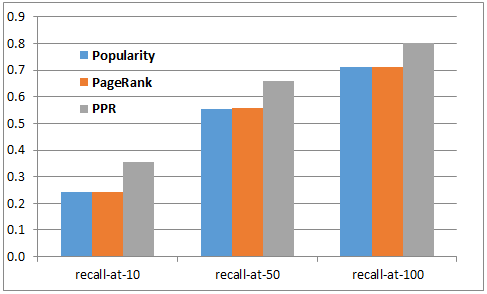
\includegraphics[scale=0.8]{figures/pop-final.png} \\
%\caption{Recall@K}
%\label{fig:minlen2remove500Recall}
%\end{subfigure}
%\begin{subfigure}[b]{0.49\textwidth}
	\centering
(b) \\
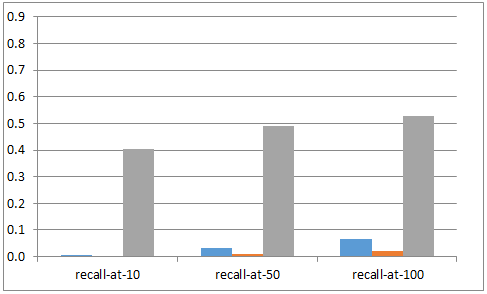
\includegraphics[scale=0.8]{figures/sans-popular-final.png}
%\caption{MRR}
%\label{fig:minlen2remove500MRR}
%\end{subfigure}
	\caption{Graph without paths without popular nodes}
	\label{fig:minlen2remove500}
\end{figure}


\begin{table}[p]
\centering
\caption{Standard deviation and Standard error of the Mean}
\label{table:std_ste}
\begin{tabular}{llcccc} \hline
	& & Recall-at-10 & Recall-at-50 & Recall-at-100 & MRR	 \\
\hline
\multicolumn{6}{c}{FULL} \\
\hline
& POP & 0.243 (0.007) & 0.555 (0.017) & 0.711 (0.012) & 0.104 (0.004) \\
& PR & 	0.243 (0.007) & 0.559 (0.016) & 0.711 (0.012) & 0.104 (0.004) \\
& PPR	& \textbf{0.354}	(0.011) & 0.660	(0.009) & 0.801 (0.004) & \textbf{0.151}	(0.006) \\
\hline
No terms & POP & 0.240 (0.009) & 0.553 (0.012) & 0.719 (0.007) & 0.101 (0.005) \\
& PR & 0.240 (0.009) & 0.563 (0.014) & 0.719 (0.007) & 0.101 (0.005) \\
& PPR	& 0.350	(0.014) & \textbf{0.665}	(0.008) & \textbf{0.809}	(0.014) & 0.146	(0.008) \\
\hline
Full path & POP & 0.065 (0.005) & 0.177 (0.010) & 0.224 (0.010) & 0.023 (0.004) \\
& PR & 0.185 (0.013) & 0.409 (0.016) & 0.538 (0.012) & 0.079 (0.010) \\
& PPR	& 0.294	(0.017) & 0.592	(0.015) & 0.708	(0.010) & 0.150	(0.008) \\
\hline
\multicolumn{6}{c}{SANS POPULAR NODES} \\
\hline
 & POP & 	0.006 (0.004) & 0.034 (0.009) & 0.065 (0.009) & 0.004 (0.001) \\
 & PR	& 0.001	(0.000) & 0.009	(0.009) & 0.022	(0.003) & 0.001	(0.000) \\
& PPR	& 0.405	(0.007) & 0.491 (0.007) & 0.527	(0.004) & 0.320	(0.005) \\
\hline
No terms & POP & 	0.000 (0.000) & 0.000 (0.000) & 0.000 (0.000) & 0.000 (0.000) \\
& PR & 	0.001 (0.002) & 0.012 (0.007) & 0.027 (0.002) & 0.001 (0.000) \\
& PPR & 	0.401 (0.027) & 0.483 (0.027) & 0.521 (0.022) & 0.322 (0.027) \\
\hline
Full path & POP & 	0.004 (0.003) & 0.019 (0.006) & 0.033 (0.007) & 0.003 (0.001) \\
& PR & 	0.032 (0.010) & 0.033 (0.010) & 0.034 (0.010) & 0.001 (0.000) \\
& PPR	& \textbf{0.496}	(0.017) & \textbf{0.575}	(0.022) & \textbf{0.602}	(0.016) & \textbf{0.415}	(0.020) \\
\hline
\end{tabular}
\end{table}


\paragraph{Impact of high-degree nodes}

A secondary question addressed concerns the graph structure. We hypothesize that in addons/users ecosystem high degree nodes insert more noise in random walk than they contribute to correct PageRank execution. In our settings, a high degree node typically means corresponds to one of the following phenomena:
\begin{itemize}
\renewcommand{\labelitemiii}{$\diamond$}
\item A highly frequent {\it term} node, which links to many {\it add-ons}. 
\item A highly popular {\it add-on}, which is associated with a large number of {\it users}. 
\end{itemize}
Such high-frequency nodes are generally known to be of low value for similarity assessment. In the graph walk schema, this implies that the probabilty mass assigned to such nodes would be distributed among a large variety of neighboring nodes in the random walk process, having little impact on the final rankings. At the same time, such nodes are likely to receive a large number of contibutions from their neighbors. The output list is likely therefore to be biased towards popular nodes.  
Notably, we wish that the Personalized PageRank distribution reflect node relevancy to the input
teleportaion vector, which simulates the user's ecosystem. The impact of high degree nodes may reduce the
influence of the original seeds.

[SELA: There is a significant improvement when we are removing high degree node and adding paths. When comparing results of graph with/without paths and without popular nodes. In this case the paths greatly improve the results (in contrast to the case when we are not removing high degree nodes - paths don't have any significant impact). Explanation:
Adding paths to the graph may contain very useful data, like nodes of type 'SKYPE\_V1', this node can connect many Skype addons that otherwise would not be connected. On the other hand, adding paths is also adding a noise to the graph. We will run the following experiment. On graph without popular nodes and with paths, we will remove the terms - we hypothesize that this will lead to similar results as in graph without paths.]

SOME OVERLAP HERE, PROCESS. High degree nodes in our graph typically represent a very popular
addons or a term. We were considering how to treat this kind of nodes,
on the one hand these nodes are part of the graph and should be
treated like all other nodes. On the other hand, given the addon
popularity, it is unfair to predict it - it is somewhat trivial. We've
conducted all of the experiments in both ways - with and without high
degree nodes. But it is our opinion that the high degree nodes should
be treated in a similar way to how the stop words in lexical analysis
are treated. Since the stop words has no interest for the prediction
algorithms it is usually removed. We've observed, see
\autoref{fig:nodes_degree_dest}, that the nodes degree distribution
follows Zipf's law distribution \textcolor{red}{Convert the graph into log scale}.


MOVE/DELETE?
\begin{itemize}
\renewcommand{\labelitemiii}{$\diamond$}
\item Graph with addons that include full path or only the addon file
  name - as described in \autoref{sec:datasets}, we have decided to
  test our method when using only addon filename as node in the graph
  and when using full addon path as node in the graph.
\item Removing high degree nodes from the graph or not. While removing
  high degree node might obviously hurt the popularity baseline
  performance.
\item Minimal number of addons user must have for running our
  prediction method. Clearly, the absolute minimum is two since when
\end{itemize}

\iffalse
\begin{figure}[t]
\centering
\begin{subfigure}[b]{0.49\textwidth}
	\centering
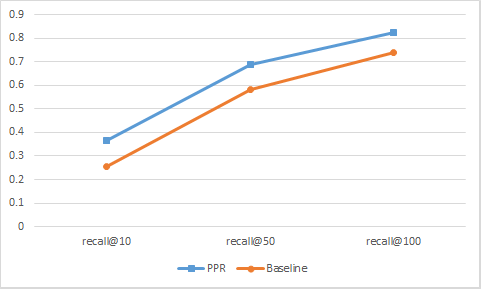
\includegraphics[scale=0.49]{figures/minlen2noremove.png}
\caption{Recall@K}
\label{fig:minlen2noremoveRecall}
\end{subfigure}
\begin{subfigure}[b]{0.49\textwidth}
	\centering
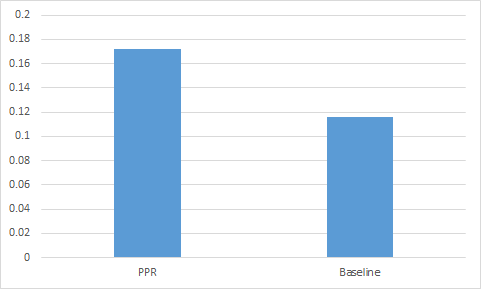
\includegraphics[scale=0.49]{figures/minlen2noremoveMRR.png}
\caption{MRR}
\label{fig:minlen2noremoveMRR}
\end{subfigure}
\caption{Graph without paths with popular nodes}
	\label{fig:minlen2noremove}
\end{figure}
\fi

In order to check how the inclusion of high degree nodes would influence
the prediction algorithm, we conducted the same experiment without removing any node
from the original graph. \textcolor{red}{Are the datapoints the same or different?} the results are shown in
\autoref{fig:minlen2noremove} \textcolor{red}{Should plot results with and  without high-degree nodes in the same graph, it is very hard to visualize the difference across figures}. We observe \iffalse similarly to \autoref{fig:minlen2noremoveRecall},\fi that Recall@10 performance has
dropped from {$\sim$}44\% to {$\sim$}36\%. On the other hand, Recall@50 and
Recall@100 ratios have improved. We believe that Recall@10 is more sensitive to the presence of popular addons compared with Recall@50 and
Recall@100, as the popular nodes occupy the top ranks, pushing relevant but less popular answer nodes to lower positions of the ranked list. However, discarding the popular nodes hurts performance in case that the missing add-on is in fact popular. Thus, overall recall@100 is higher in the case that they are indeed included. 

\par Given the differences between the algorithms scores, it is a good
place to mention the standard deviation (SD) and the standard mean error (SME) of the experiments, see
\autoref{table:std_ste}. \textcolor{red}{What is it showing? detail in text and in caption. Discuss the findings.}
\begin{table}[t]
\centering
\caption{Standard deviation and Standard error of the Mean}
\label{table:std_ste}
\begin{tabular}{|c|c|c|c|} \hline
 & Recall@10 & Recall@50 & Recall@100\\ \hline
MEAN & 0.358904 & 0.661086 & 0.80593\\ \hline
SD & 0.001773 & 0.002601 & 0.005279\\ \hline
SME & 0.001024 & 0.001502 & 30.003048\\ \hline
\end{tabular}
\end{table}

\paragraph{Impact of term modeling in the graph}

As discusses earlier, we include {\it terms} in the graph, so as to model term-based lexical similarity between co-referent (or generally similar) add-on descriptions. We are thus interested in evaluating the contribution of term modeling for our task.

\iffalse
\begin{figure}[t]
\centering
\begin{subfigure}[b]{0.49\textwidth}
	\centering
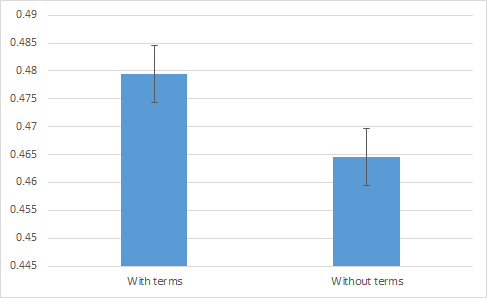
\includegraphics[scale=0.49]{figures/5addonswithoutTermsComp.png}
\caption{With/without term nodes with paths without popular nodes}
\label{fig:with_without_terms5}
\end{subfigure}
\begin{subfigure}[b]{0.49\textwidth}
	\centering
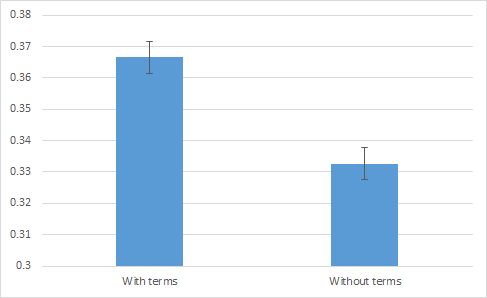
\includegraphics[scale=0.49]{figures/2addonswithoutTermsComp.png}
\caption{With/without term nodes without paths with popular nodes}
\label{fig:with_without_terms2}
\end{subfigure}
\caption{Comparing graph with/without addon paths}
	\label{fig:with_without_terms}
\end{figure}
\fi

As shown in
\autoref{fig:with_without_terms}, including term nodes improves the prediction.\textcolor{red}{a. Why not show recall@k here? also, need to describe what the figure shows verbally.} Moreover, experiments using a graph variant that included {\it add-ons} and {\it term} nodes only, showed poor performance. We suggest the following explanation to this result. In the graph, add-on nodes are typically connected to a large number of {\it user} nodes, and only to very few {\it term} nodes. To illustrate this, consider some arbitrary add-on with a short description, linking to three {\it term} nodes, and a medium user set neighborhood consisting of 200 {\it user} nodes. 
The transition operation of the applied graph walk assumed uniform distribution over each node's neighbors. Therefore, the total probability flow through the {\it term} nodes is relatively small. \iffalse Given that we are running Personalized pagerank and supposedly many users are the same for the vector of current addons, than most of
the weight will go via the users and terms will get very small weight
to traverse. \fi While term node might be connected to many other
addons - it almost doesn't get any weight from them since we are
running Personalized PageRank and not regular PageRank most of the
weight is concentrated in the personalized vector - which contains
only current user addons and not terms.

As mentioned at \autoref{sec:method}, the addons data as collected
from the users refers to addons usually by full file system path,
e.g. C:/Program Files/Skype/skype1.dll, While breaking this addon to
term nodes this would create four nodes $C$,$Program Files$, $Skype$
and $skype1$. In \autoref{fig:minlen2noremove} and
\autoref{fig:minlen2remove500}, we have chosen to remove the file
system path from addon, hence the NoPath abbreviation, so we actually
would have only one node $skype1$. We have also conducted
\autoref{fig:minlen2noremove} experiment while not removing file
system path from addon. The results are shown at
\autoref{fig:minlen2noremoveWithPaths}.

\iffalse
\begin{figure}[t]
\centering
\begin{subfigure}[b]{0.49\textwidth}
	\centering
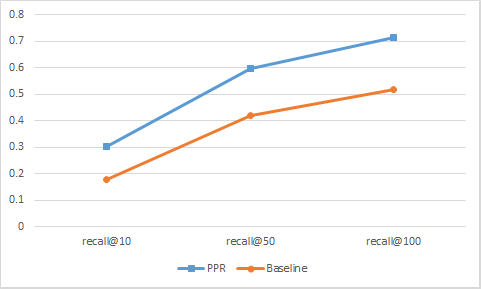
\includegraphics[scale=0.49]{figures/minlen2noremoveWithPaths.png}
\caption{Recall@K}
\label{fig:minlen2noremoveRecall}
\end{subfigure}
\begin{subfigure}[b]{0.49\textwidth}
	\centering
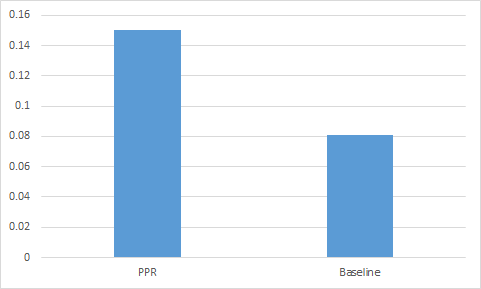
\includegraphics[scale=0.49]{figures/minlen2noremoveWithPathsMRR.png}
\caption{MRR}
\label{fig:minlen2noremoveMRR}
\end{subfigure}
\caption{Graph with paths with popular nodes}
	\label{fig:minlen2noremoveWithPaths}
\end{figure}
\fi

If we compare the results of the same run, as shown in
\autoref{fig:with_without_paths_noremove}, we observe that adding
addons paths hurts the performance, this can support our claim that
high degree nodes, which obviously added when adding addons paths,
disturb the PPR weight propagation from the real missing addons
nodes. Interestingly, adding addons paths but removing high degree
nodes improves the performance of our algorithm, see
\autoref{fig:with_without_paths_remove500}. These two experiments,
shown in \autoref{fig:with_without_paths}, support our claim that high
degree nodes should be removed to improve prediction quality. Since,
once they are removed, addition information about the user, like it
paths, contributes to understanding and predicting its ecosystem
state.

\iffalse
\begin{figure}[t]
\centering
\begin{subfigure}[b]{0.49\textwidth}
	\centering
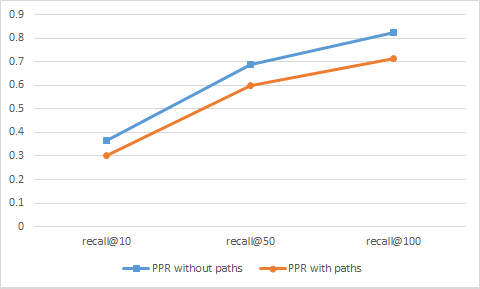
\includegraphics[scale=0.49]{figures/minlen2noremoveCompPaths.png}
\caption{With/without addon paths with popular nodes}
\label{fig:with_without_paths_noremove}
\end{subfigure}
\begin{subfigure}[b]{0.49\textwidth}
	\centering
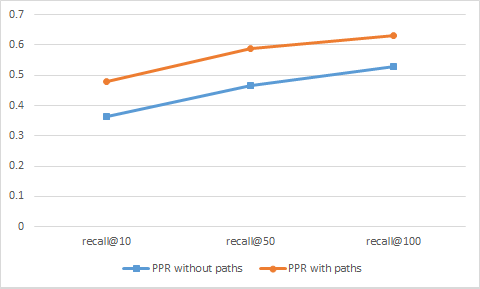
\includegraphics[scale=0.49]{figures/minlen5remove500CompPaths.png}
\caption{With/without addon paths without popular nodes}
\label{fig:with_without_paths_remove500}
\end{subfigure}
\caption{Comparing graph with/without addon paths}
	\label{fig:with_without_paths}
\end{figure}
\fi

As we have mentioned earlier, in order for our prediction algorithm to
run, we require that user has at least two add-ons. At
\autoref{fig:addonsNumberGraph},we are showing the affect number of
addons that user have pre-installed on the algorithm accuracy. The
\autoref{fig:addonsNumberGraph} graph shows that, while the prediction
algorithm still performs on any number of pre-installed, its accuracy
decreases as the number addons that user has, growth. One possible
explanation to this behavior could be - if user addon is predicted,
i.e. receives its PageRank score, mainly from other users that have a
similar ecosystem - that the lesser addons user has the more unique
its ecosystem.

\begin{figure}[p]
\centering
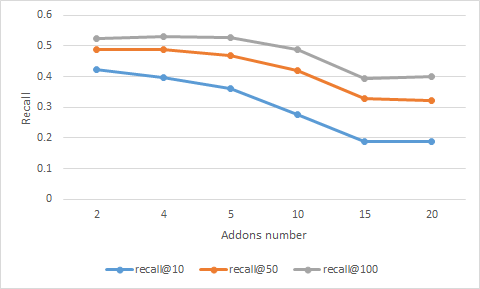
\includegraphics[scale=1,angle=0]{figures/addonsNumberGraph.png}
\caption{Effect of addon number on prediction accuracy}
\label{fig:addonsNumberGraph}
\end{figure}



We have also verified that user nodes are crucial for the prediction
algorithm, as shown in \autoref{fig:nouserNoremove}.

\begin{figure}[h]
\centering
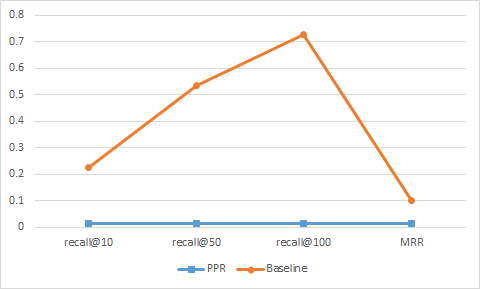
\includegraphics[scale=.8,angle=0]{figures/nouserNoremove.png}
\caption{Effect of user nodes on prediction accuracy}
\label{fig:nouserNoremove}
\end{figure}


\section{Discussion}
Our prediction algorithm performs best on full graph when highly
connected nodes are removed, removing very highly connected nodes
improves PPR convergence and reduces the noise in random walk.
Moreover, users that are having only two addons eases the prediction,
which intuitively makes sense since the PPR personalization vector
contains only one node. In experiment shown in
\autoref{fig:addonsNumberGraph}, you can observe that picking users
with higher number of pre-installed addons reduces the algorithm
performance but still performs well. In experiment shown in
\autoref{fig:with_without_terms}, you can observe the importance of
term nodes, they improve connectivity between similar addons and thus
improves our prediction rate. An obvious observation can be made from
experiment shown in \autoref{fig:nouserNoremove}., graph without user
nodes are almost not possible for recommender to find a missing addon
node.


\chapter{PPR-based analysis of addon coexistence}
\label{chap:Symbiosis}

In this chapter, we investigate the addon coexistence phenomenon. We observe that some addons tend to coexist well with other addons, i.e. when addons of one company are installed on a user's PC, addons of another company have greater chances to be installed on the same machine.  This phenomenon often occurs when addons of some companies are distributed via third parties: addon installation is proposed to a user as a part of some other product installation process, for example, while the user installs Skype, the installation process suggests also installing Skype's `Click to Call' addon in all browsers. Another example is Google Toolbar: when the data for this paper was collected, Google distributed its toolbar in conjunction to installation of other products, such as Firefox or Winrar.

The opposite effect to coexistence can be observed as well: addons of one company have lower chances to exist on a machine if addons of another company are installed on this machine. For example, \emph{Avira AntiVirus}, which develops addons for all browsers, treats \emph{iMesh} addons as threats and removes them from the computer.

Companies that distribute browser addons are engaged in partnerships or compete with each other, such that the Web browser becomes a complex ecosystem similar in its characteristics to the biological environment of the nature. To illustrate this analogy, let us say that addon distributors correspond to biological species. An instance of an addon distributed by company $A$ can be viewed as a subject of species $A$ that coexists in the browser ecosystem with other subjects of the same or different species. Naturally, those subjects can live in symbiosis or in conflict with each other. We observe situations when addons of some companies get installed on a machine together with addons of other companies, which is analogous to a natural migration process when subjects of different species travel together. We also observe clash situations when an addon gets installed on a machine and ``kicks out'' addons of other companies, similarly to a competition phenomenon between different species in the nature. The user (the computer owner) is also playing an important role in the addon ecosystem: some users ``hunt down'' and remove addons that occasionally appear in the computer's browser; other users are more tolerant -- they let addons live in the browser for a long time and do not mind more addons to be added over time.

Needless to say, the life cycle of the addon ecosystem is mostly obscure for an outside observer. While some symbiosis effects are fairly visible to the users (e.g., an addon is prompted to be installed during an installation processes of another addon or software product), many other effects are hidden (e.g., undisclosed agreements between addon distributors) or implicit (two addons are statistically prone to coexistence). Clash effects, on the other hand, are almost always invisible. Besides a few well known conflicts between competing addon distributors that were widely covered in mass media\footnote{\url{http://finance.yahoo.com/news/babylon-shares-jump-yahoo-sticks-125203474.html}}, the competition is kept away from the eyes of general public. In this chapter, we disclose some of these effects and shed light on the entire addon ecosystem. 

The ability to detect and analyze a clash or symbiosis between addon distributing companies could turn handy for addon owners. 
A typical company that builds its business around developing and distributing addons (via a webstore, for instance), can benefit from information about a clash between their and someone else's addons, in four different ways.
First, such a clash may imply that the user prefers someone else's addon over their addon, so there might be a way to compare the two addons and  learn how to improve their value proposition. 
%Most probably, the user prefers the competitor's addon for a specific reason. In the Web browser ecosystem, identifying one's competitor is not an easy problem --- the clash information can help to solve this problem.
Second, the clash could mean that a newly installed addon is hostile to other addons in an illegal way, i.e. it is the addon --- and not the user ---- that uninstalls or sabotages another addon. Then, the distributor of the removed addon could report an abuse to the webstore owner.

Third, an addon developing company can ask a third-party distributing company not to install their addon on a machine that keeps the hostile addon. Since in most cases addon developers are paying distributors per install, this could decrease the developers' costs and improve their profits in a long run.
Fourth, a clash can occur between addons of seemingly non-competing companies. This can happen when something goes wrong in the distribution process and the problem slips off the company's radar. The addon ecosystem is complex enough to make the distribution monitoring barely possible. If an unintended clash gets detected, the owner of the affected addon can contact the owner of the hostile addon and ask to act.

To the best of our knowledge, this thesis is the first research study of the addon ecosystem in the Web browser. This is a true Big Data study as we analysed Web browsers of close to a million users. Both addon developers and computer security companies can benefit from this study and its conclusions. In the rest of this chapter, we will describe the setup of our empirical analysis, in particular, the reasons behind its design choices. We will provide background information and cover the history of this project starting with preliminary experimental efforts we made before coming up with our final experimental design. We will then present our findings: the identified symbiosis and competition relationships. We will conclude this chapter with a discussion of the results.

\iffalse
Another observation we've made, is that company addons tend to collocate together - we succeeded detecting company addon without any clues in its name that it belongs to any specific company.
\fi

\section{Experimental setup}
We chose nineteen companies (see~\autoref{table:companies_list}) among well-known addon distributors. These are ``famous'' companies that are distributing addons and toolbars. Their addons are distributed through the installation process of third-party software products, like Adobe Reader. Most of the time, during the software installation, an opt-out check box is presented to the user per addon to be installed. If the user chooses to uncheck the box, the addon will not get installed. However, many users click through the installation process without reading the small font, and when the process is completed the users discover they installed something they did not intend to. 

Anti-virus and anti-malware software aim to prevent unintentional addon installation. For example, in 2013, Avast Anti Virus published a list of top ten companies that were distributing their addons via third-party software installations \footnote{\url{https://blog.avast.com/2013/03/20/avast-browser-cleanup-at-work/}}. Surprisingly, the list published by Avast in 2015 is very similar to their 2013 list --- many of these companies are in our list as well~(\autoref{table:companies_list}). Back in 2013, Avast identified over 3,300,000 different browser extensions for three major browsers. They also noticed that ``A lot of toolbars are available in different variants. These variations affect mostly the name''. Some anti-virus companies are not only fighting unintentional addon installations but also distributing their addons and toolbars in a similar way. For example, AVG Anti Virus company distributes an AVG Security Toolbar which is detected by Avast Anti Virus as malware. 

In Avast recent blog post from July 9th 2015, they describe the addon ecosystem of a user's Web browser. They mention that one of the major characteristics of the ecosystem is that ``the addons fight against each other'' \footnote{\url{https://blog.avast.com/2015/07/09/top-10-most-annoying-browser-toolbars/}}.
Based on Avast statistics on forced removals of competing toolbars, some companies from our list are among the top ten offenders. For example, Conduit performed more than 13,000,000 removals of their competitors' toolbars, ASK removed 11,000,000 toolbars and other companies were not far behind. Interestingly, Avast itself uses the same practice \footnote{\url{http://techdows.com/2012/11/avast-comes-bundled-with-google-toolbar.html}}: ``Avast is contradicting itself. Their latest product offers a built-in feature to rid your browser of toolbars, while offering a toolbar when installing their software.''


% Please add the following required packages to your document preamble:
% \usepackage{booktabs}
\begin{table}[h]
\centering
\caption{Companies list}
\label{table:companies_list}
\begin{tabular}{@{}lll@{}}
\toprule
{\bf Company name} & {\bf Example Product}               & {\bf Description}               \\ \midrule
ASK                & Ask Toolbar                 & Advertisement/Search company    \\
AVG                & AVG Safe Search add-on      & AntiVirus/Advertisement company \\
Avira              & Avira Browser Safety        & AntiVirus company               \\
Babylon            & Babylon Toolbar             & Advertisement/Search company    \\
Blekko             & Blekko Toolbar              & Advertisement/Search company    \\
Conduit            & Conduit Toolbar             & Toolbar provider company        \\
Google             & Google Toolbar              & Advertisement/Search company    \\
Hotspot Shield     & Hotspot Shield VPN          & Security company                \\
iMesh              & iMesh Search                & Advertisement/Search company    \\
Incredimail        & MyStart by Incredimail      & Advertisement company           \\
Kaspersky          & Kaspersky Protection Plugin & AntiVirus company               \\
Montiera           & Montieara Toolbar            & Toolbar provider company        \\
Norton             & Norton Toolbar              & AntiVirus company               \\
Softonic           & Softonic Web Search         & Advertisement company           \\
SpeedBit           & Video Accelerator           & Software company                \\
SweetIM            & SweetIM Toolbar             & Advertisement/Search company    \\
Trend Micro        & Trend Micro Toolbar         & AntiVirus company               \\
Zone Alarm         & Zone Alarm Toolbar          & AntiVirus company               \\ 
Zugo               & Search Toolbar              & Advertisement company           \\ \bottomrule
\end{tabular}
\end{table}

\iffalse
At first, we have tried to classify add-ons clash with Support Vector machine, but we saw no signal and the SVM could not converge. [Need much more info here - RON, UPDATE: did we actually use SVM for predicting clash? I think we used SVM to predict an addon survival which is mainly affected by the user behavior. Anyhow, I would love to see a paragraph explaning what we did back then.]
\fi

\subsection{Preliminary Experimentation Efforts: Addon Survival Prediction}
Initially, our experimentation efforts were concentrated on addon \emph{survival prediction}. On an example of one addon development company, Speedbit, we aimed to identify Web browsers whose ecosystem allowed Speedbit addons to survive for an extended period of time, in contrast to those browsers where Speedbit addons tended to get uninstalled quickly. We approached the survival prediction task within the Machine Learning framework of \emph{binary classification} [RON:citation needed]. In binary classification, a prediction model is trained on labeled data of two classes: positive instances and negative instances. We constructed our training data as follows: browsers in which Speedbit addons survived for three or more days were considered positive instances---all other browsers were considered negative instances. We used the popular libSVM tool [RON:citation needed] to train our prediction model.
%The 3 days threshold, it turns out that the toolbar doesn't survive that well - the number of users for whom the toolbar survived 3 or more days is less than 10 percentage of all users.
We split our dataset to $2/3$ training set and $1/3$ test set (uniformly at random). Since we had about 900,000 instances in our dataset, our training set consisted of about 600,000 instances. This training set turned out to be too large for modern non-parallelized binary classification systems. After a few unsuccessful attempts to train the model on the entire training set, we decreased its size by taking all positive instances and a random sample of 1/3 of negative instances.

\iffalse
Running training libsvm on the new samples took one hour.
optimization finished, iter = 41654
nu = 0.706971
obj = -196797.924484, rho = 1.994601
nSV = 40041, nBSV = 39227
Total nSV = 40041
Then we've decided to find another way to represent our data.

In \autoref{chap:user_ecosystem} our algorithm's viewpoint was set of add-ons of a specific user set of add-ons - we were viewing user add-ons as its ecosystem and predicting a missing addon according to it. Now, we are aiming to investigate symbiotic relations between companies that are producing a variety of add-ons, the algorithm viewpoint is the symbiotic relationships between ecosystems created by add-ons manufactures.
\fi

\section{Experimental design}

In ~\autoref{chap:user_ecosystem}, we investigated the addon ecosystem on the individual level: if a subject (an addon) is artificially extracted from a web browser of a specific user, the browser ecosystem ``knows'' which subject is missing. In this chapter, in contrast, we analyze the behavior of \emph{species}, i.e.~addon developing companies. In the new setting, we first need to reveal which addons belong to which companies. An addon company most often distributes many addons --- hundreds or even thousands. For example, \emph{Kaspersky URL Advisor Firefox addon} and \emph{Kaspersky Protection Chrome extension} are developed by the same company, so we say that they belong to the same species. Often, the same addon has different names --- it is not easy to infer that addons with different names are in fact the same addon. We do not aim to infer that --- instead, we are concerned with mapping addon names to company names. Also, it is important to mention that addons bear characteristics of a machine on which they are installed. For example, the file-system path of an addon on a specific machine may or may not be unique among all addons we observe in this study: a user can choose to install an addon at a non-standard location in his/her machine's file system, or stick to a default location instead.

As discussed in Section~\ref{sec:methods}, an addon is represented in our system by three data attributes: the addon's name, the full file-system path of its installation, and a textual description. Each one (or any two but not all three) of the attributes may be empty. To infer which addon belongs to which company, we first apply a simple heuristic of detecting the company name within the three attributes of an addon. The rationale behind this is that the default path of an addon package installation often contains the company's name. If a user does not choose to change the default option, the company name will be detected in the addon's path. In addition, the name and the description fields may contain the company name as well, see \autoref{table:addon_desc} for an example.

% Please add the following required packages to your document preamble:
% \usepackage{booktabs}
\begin{table}[h]
\centering
\caption{An example of a company's name contained in an addon's path or description}
\label{table:addon_desc}
\begin{tabular}{@{}|l|l|@{}}
\toprule
Addon installed in a folder containing the company name & C:\textbackslash{Program Files (x86)}\textbackslash{Kaspersky Lab}\\ & \textbackslash{Kaspersky Internet Security 2012}\textbackslash{avp.dll} \\ \midrule
Addon description containing the company name & Kaspersky Protection extension \\ \bottomrule
\end{tabular}
\end{table}

After applying the company name search heuristic, we realized that representations of many addons that belong to companies from our list~\autoref{table:companies_list} do not in fact contain the company name. For example, an addon $tbbaby.dll$ doesn't contain company name in any of its attributes, but does belong to Babylon\footnote{\url{http://www.shouldiremoveit.com/Babylon-English-Toolbar-31094-program.aspx}}. 
We propose the following procedure, see algorithm \autoref{alg:find_addon_species}, for mapping this kind of addons to their owners. 

In Chapter~\autoref{chap:user_ecosystem}, we applied a Personalized PageRank (PPR) based algorithm for identifying a missing addon in a browser of a specific user. We proposed a method that took the entire set of the user's addons as a query input to PPR and produced the output of a ranked list of all addons in the system. We hypothesized that the missing addon would end up among the top addons in the ranked list. Our hypothesis was proved correct.

We apply a similar method here, for mapping addons to their manufacturer companies. As a query for the PPR algorithm, instead of the set of addons existing in a user's browser, we now provide a set of addons that are known to belong to a company. We hypothesise that an addon that belongs to that company, and is not in the query, would ``pop-up'' in the ranked list. By ``popping-up'' we mean that the addon would be ranked closer to the top of the list, relatively to its original rank in the (non-personalized) PageRank. First, we run the not personalized PageRank on the entire graph, and use the rank of each addon as the baseline position. For each company, we then run the Personalized PageRank and identify addons that drastically changed their position in the ranked list. For example, if an addon was at a rank of 15 in the non-personalized PageRank and moved to the rank of 14 in the PPR, we do not take it into account as its rank did not dramatically change. In contrast, if an addon was at a rank of 100 in the non-personalized PageRank and moved to the rank of 10 in the PPR, we consider it as a candidate to manual examination. For each addon that ``popped-up'' in the ranked list of a specific company's PPR, we manually validate that the addon actually belongs to the company. 

We perform the procedure described above iteratively: after we discover addons that belong to a company, we add them to the query and rerun the PPR with the extended query. We stop the process once there are no more addons that dramatically change its rank. It turned out that two iterations were enough for the process to converge. Using this process, we found 24 [SELA: Recheck the number] addons that ``popped up'' in the PPR ranked lists of companies from~\autoref{table:companies_list}. In a manual check of these 24 addons, we saw 100\% precision: there was not one single addon we checked that did not after all belong to the company in the query. 

\begin{algorithm}[!t]
\caption{Finding addon relation to Company}
\label{alg:find_addon_species}
\begin{algorithmic}[1] 
\REQUIRE Graph $G$, teleportation vector $v$, company name $n$
\STATE Run Personalized PageRank on graph $G$, with seed node from $v$.
\STATE Rank the addons according to $PPR_gscore$, i.e. the Personalized PageRank scores after run
\FOR{each addon node}
\STATE Compare $PPR_gscore$ with $PR_gscore$
\IF{$PPR_gscore$ $\gg$ $PR_gscore$}
\STATE This addon could be related to the company - check manually
\ENDIF
\ENDFOR
\end{algorithmic}
\end{algorithm}

An example for an addon that drastically changed its score is the addon named \emph{tbmyba.dll}, the addon's $PR_gscore$ was 1200, and the $PPR_gscore$ turned to be 15 when using seed nodes related to Babylon. Indeed, we found that this addon belongs to Babylon\footnote{\url{http://www.file.net/process/tbmyba.dll.html}}.

The success of this process reveals an interesting phenomenon: it turns out that there is a ``community'' of addons of the same species, and this community can be discovered via the Personalized PageRank weight propagation that starts with already known community members. One possible explanation for this phenomenon would be that it is a common practice for a company to offer a few of its addons for installation at the same time. For example, while Babylon is installing an Internet Explorer addon, it might also install a Chrome extension. Even if we manage to map the Internet Explorer addon to Babylon using the simple name matching procedure, the Chrome extension might not contain any attribute that would qualify it as related to Babylon. Still, our algorithm would discover it in a similar way it discovered a missing addon for a specific user. 
Another explanation may come from the \emph{collaborative filtering} theory: users who have many addons in common might also have different addons of the same company --- such addons will therefore be located in a close proximity of each other in the PageRank graph.

Now that we linked addons with their species (that is, their manufacturer companies), we are ready to analyze relations between the addon species in World Wide Web ecosystem. The following algorithm~\autoref{alg:collect_addon_data} summarizes our methodology. 
For each company from our list, we construct the PPR query to contain all the company's addons. The PPR output is the ranked list of all addons in the graph. Our goal is to find out addons of which companies ``pop up'' in the PPR as compared to non-personalized PageRank. If we identify a company whose addons are universally improving their rank in the PPR of another company, we may conclude that the two companies are engaged in a partnership. Using the ecological language, we call it \emph{symbiosis}. We also expect addons of some companies to ``drop down'' the PPR ranked list, in comparison to the regular PR ranked list. We can suggest that two companies \emph{clash} if many addons of one company drop down in the PPR of another company.

\begin{algorithm}[!t]
\caption{Collecting data for each add-on}
\label{alg:collect_addon_data}
\begin{algorithmic}[1] 
\REQUIRE Graph $G$, Companies $COMP$
\STATE Run PageRank on graph $G$
\FOR{company $c\in COMP\ $}
\STATE Define personalization vector $v$, with seed nodes as all addons $\in COMP\ $
\STATE Execute Personalized PageRank
\STATE Rank all addons according to the PPR score
\STATE Store the results [RON: I guess we need something more sufficient than storing the results]
\ENDFOR
\end{algorithmic}
\end{algorithm}

\section{Analysis}
\subsection{Symbiotic Relationships}
\label{sec:symb_relations}

Addon ranking obtained by the ordinary (non-personalized) PageRank corresponds to the unbiased and undisturbed addon ecosystem in which every addon bears its relative importance value with respect to the others. Once the personalized PageRank is applied, the ecosystem is disturbed with artificial preference of some of its elements. The artificial disturbance causes the entire ecosystem to adjust to the new condition, and such a adjustment reveals characteristics of the ecosystem that would not be visible in the original, undisturbed state. 

When all addons of a particular company comprise the PPR query, it would be natural to expect the company's addons popping up in the ranked list. Other addons that are closely related to the addons of the query company might then follow the company's addons in their way to the top of the ranked list. The beauty of personalized PageRank is in the fact that the essence of the relationship between the addons does not have to be disclosed a priori, nor explicitly modeled. This implies that hidden, invisible relationships between addon manufacturers can be discovered in the process.

Our research hypothesis is that addons that pop up in the PPR ranked list belong to a company $C_i$ that is involved in a symbiotic relationship with the query company $C_q$. Our goal is to reveal such a relationship based on the $C_i$'s addon behavior as a reaction to the PPR disturbance of the addon ecosystem. Since companies usually maintain many addons, we cannot expect any company to have all its addons universally popping up in the ranked list once PPR is applied. Obviously, some addons would pop up higher than the others, while some addons might not change their rank substantially, or even drop down the ranked list. If we measure the rank change of addons that belong to $C_i$, we could make a conclusion about the probability of a symbiotic relationship between $C_i$ and $C_q$.

There are two factors that affect the significance of the addon's rank change:
\begin{enumerate}
\item \textbf{Length of the leap.} Obviously enough, the longer is the addon's leap from the original rank (in non-personalized PR) to the new rank (in PPR), the more significant the rank change is.
\item \textbf{The (final) PPR rank.} The length of the leap is not the only significance measure. Intuitively, if an addon jumps from rank 10,000 to rank 1000, such a jump is less significant than if the addon jumped from rank 100 to rank 10. The explanation is simple: an addon at a rank 10,000 was most probably not important, and a big change in its rank would not make it significantly more important. In contrast, an addon that moved to the 10th place cannot be ignored.
\end{enumerate}

We are interested in the change of rank of the company, as aggregated over the set of its addons' ranks. In a search for a formula that would aggregate the behavior of all the company's addons, we make the following observation: if an addon is rare (i.e.~installed on just a few browsers), then the change in its rank --- even a significant one --- might have little effect on the behavior of the company in whole. For example, if an addon moves from rank 10,000 to rank 10, but is installed on 10 browsers only, its effect on the aggregated rank of the company would be less significant than, say, a change in rank from 100 to 50 of an addon that is installed on 10,000 browsers.

The potential complexity of addon rank aggregation over the three parameters listed above (length of the leap. the final rank, and the addon frequency) makes us search for simplification. Since an addon's rank is determined by the order of all addons when sorted over their PR (or PPR) \emph{scores}, we observe that an addon score is a better measure of the addon's importance than its rank. For example, if an addon's score was 5 in the non-personalized PR, and got increased to 10 in PPR, while there were no other addons with scores as high as 5, then the rank of the addon would not change, so the significance of the score change would be completely ignored when taking into account addon ranks only. In addition, the change in the addon's rank is affected by the change of other addons' ranks, while the change of the addon's score can be taken independently from the other addons' score change. Therefore, we decide to focus on addon PR scores rather then on ranks. Now, there are only two parameters that need to be taken into account for measuring a company's ``importance'': the PR (or PPR) scores of its addons, and their frequencies in the dataset.

We estimate the ``importance'' of company $C$ by its \emph{expected} PR score, which is the weighted sum of PR scores of the company's addons. Let us denote $s_i$ the PR score of addon $a_i$ that belongs to $C$. The expected score $S_C$ (of the company $C$) will then be:
$$
S_C = \sum_{a_i \in C} p_i s_i
$$
where $p_i$ is the probability of drawing addon $a_i$ out of all $C$'s addons. Specifically, we define $p_i = freq(a_i) / freq(C)$, where $freq(a_i)$ is the frequency of addon $a_i$ in terms of the number of user browsers on which $a_i$ is installed; $freq(C)$ is the sum of all its addons' frequencies.

%After running the PPR with all addons of a company $C_q$ in the query, we first remove $C_q$'s addons from the ranked list in order to make a clean experiment: depending on the number of addons $C_q$ is maintaining --- and their original PR ranks --- their PPR ranks can significantly affect the change in ranks of other addons. We want to eliminate this influence and focus on the rank change of the other companies' addons. That is why we remove $C_q$'s addons both from the PPR ranked list and from the original PR ranked list.

%We examine the top 100 addons (after removing $C_q$'s addons), and compare their ranks to their original PR rank. For each company other than $C_q$, we [RON:Here] only addons that have more than 100 users, only nodes that belong to the companies of interest, 

%Add the formula that describes relative jump. Expected score

% Please add the following required packages to your document preamble:
% \usepackage{booktabs}
\begin{table}[h]
\centering
\caption{PageRank scores}
\label{table:pagerank_scores}
\begin{tabular}{@{}llll@{}}
\toprule
Company name   & \#addons & Total PageRank score & Average PageRank score \\ \midrule
ASK            & 229038   & 8.79139              & 0.97682                \\
AVG            & 131337   & 8.50985              & 0.38681                \\
Avira          & 10624    & 0.45046              & 0.15015                \\
Babylon        & 191386   & 23.22184             & 1.10580                \\
Blekko         & 14381    & 0.43715              & 0.06245                \\
Conduit        & 21671    & 0.51959              & 0.07423                \\
Google         & 187455   & 13.40115             & 1.11676                \\
iMesh          & 23954    & 7.05849              & 0.64168                \\
Incredimail    & 76198    & 5.79210              & 0.48268                \\
Hotspot Shield & 54675    & 2.00773              & 0.28682                \\
Kaspersky      & 47793    & 2.65493              & 0.53099                \\
Montiera       & 809      & 0.01752              & 0.01752                \\
Norton         & 53826    & 3.22903              & 0.40363                \\
Zugo           & 5169     & 0.23296              & 0.02912                \\
Softonic       & 29410    & 0.82528              & 0.05158                \\
SpeedBit       & 484676   & 59.02209             & 2.81058                \\
SweetIM        & 84871    & 2.49227              & 0.49845                \\
Trend Micro    & 10325    & 0.56126              & 0.05102                \\
Zone Alarm     & 3597     & 0.10790              & 0.01541                \\ \bottomrule
\end{tabular}
\end{table}  

\iffalse
A personalized PageRank vector is the stationary distribution of a random walk that, with probability $\alpha$ follows a step of a random walk and with probability $(1-\alpha)$ jumps back to a seed node. When there are multiple seed nodes, then the choice of the seed node is uniformly random. Thus, nodes close to the seed are more likely to be visited and get a higher rank. Recently, such techniques were shown to produce communities that best match communities found in real-world networks~\citep{abrahao2012separability}. Putting company nodes as the only seed nodes in personalized PageRank will grant a higher score to the company addons and the addons that are related in some way to this company. Our hypothesis is that nodes of the company that are having symbiotic relation with the seed nodes company will also get a higher score because of its relatedness to the symbiosis company.
\fi

As described above, we aggregate PageRank scores of all company addons and compare between companies based on the aggregated score. For exach company $C_q$ in the PPR query, we rank all the other companies of our interest according the the company's aggregated PPR score. We also maintain the ranked list of companies sorted by their aggregated (non-personalized) PR scores. For each $C_q$, we compare the two ranked lists of companies. If a company $C_i$ ``pops up'' closer to the top of the $C_q$'s PPR ranked list of companies, as compared to the original (non-personalized) ranked list of companies, we conclude that $C_i$ and $C_q$ are in a symbiotic relationship. See~\autoref{fig:symbiotic_pagerank} for the summary of our results.

%\autoref{fig:incredi_sym_blekko} illustrates a symbiosis between Incredimail and Blekko. This discovery has an online reference\footnote{\url{http://www.im-infected.com/hijacker/blekko-search.html}}. As shown in \autoref{fig:blekko_sym_incredi}, this relationship is mutual: Blekko also benefits from this symbiosis, as well as Incredimail. 

IncrediMail (Perion) and Conduit

Avtiviruses bring other antiviruses down

Zugo, SearchToolbar and SweetIM going together

The same relationship is detected for Babylon and Conduit, see \autoref{fig:babylon_sym_conduit}, and again there is more than one online resource indicating the same. For example, Babylon addon named \emph{tbmyba.dll} is a Conduit Toolbar component\footnote{\url{http://www.file.net/process/tbmyba.dll.html}}. In fact, Conduit is known as a Toolbar manufacturer for other companies.

\begin{figure}[h]
\centering
\begin{subfigure}[b]{0.49\textwidth}
	\centering
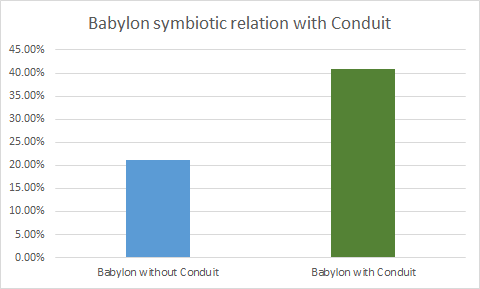
\includegraphics[scale=0.49]{figures/babylon_sym_conduit.png}
\caption{Babylon symbiotic relationship with Conduit}
\label{fig:babylon_sym_conduit}
\end{subfigure}
\begin{subfigure}[b]{0.49\textwidth}
	\centering
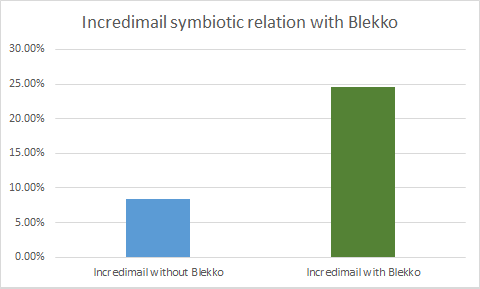
\includegraphics[scale=0.49]{figures/incredi_sym_blekko.png}
\caption{Incredimail symbiotic relationship with Blekko}
\label{fig:incredi_sym_blekko}
\end{subfigure}
\caption{Symbiotic relationship between companies}
	\label{fig:symbiotic_pagerank}
\end{figure}

\begin{figure}[h]
\centering
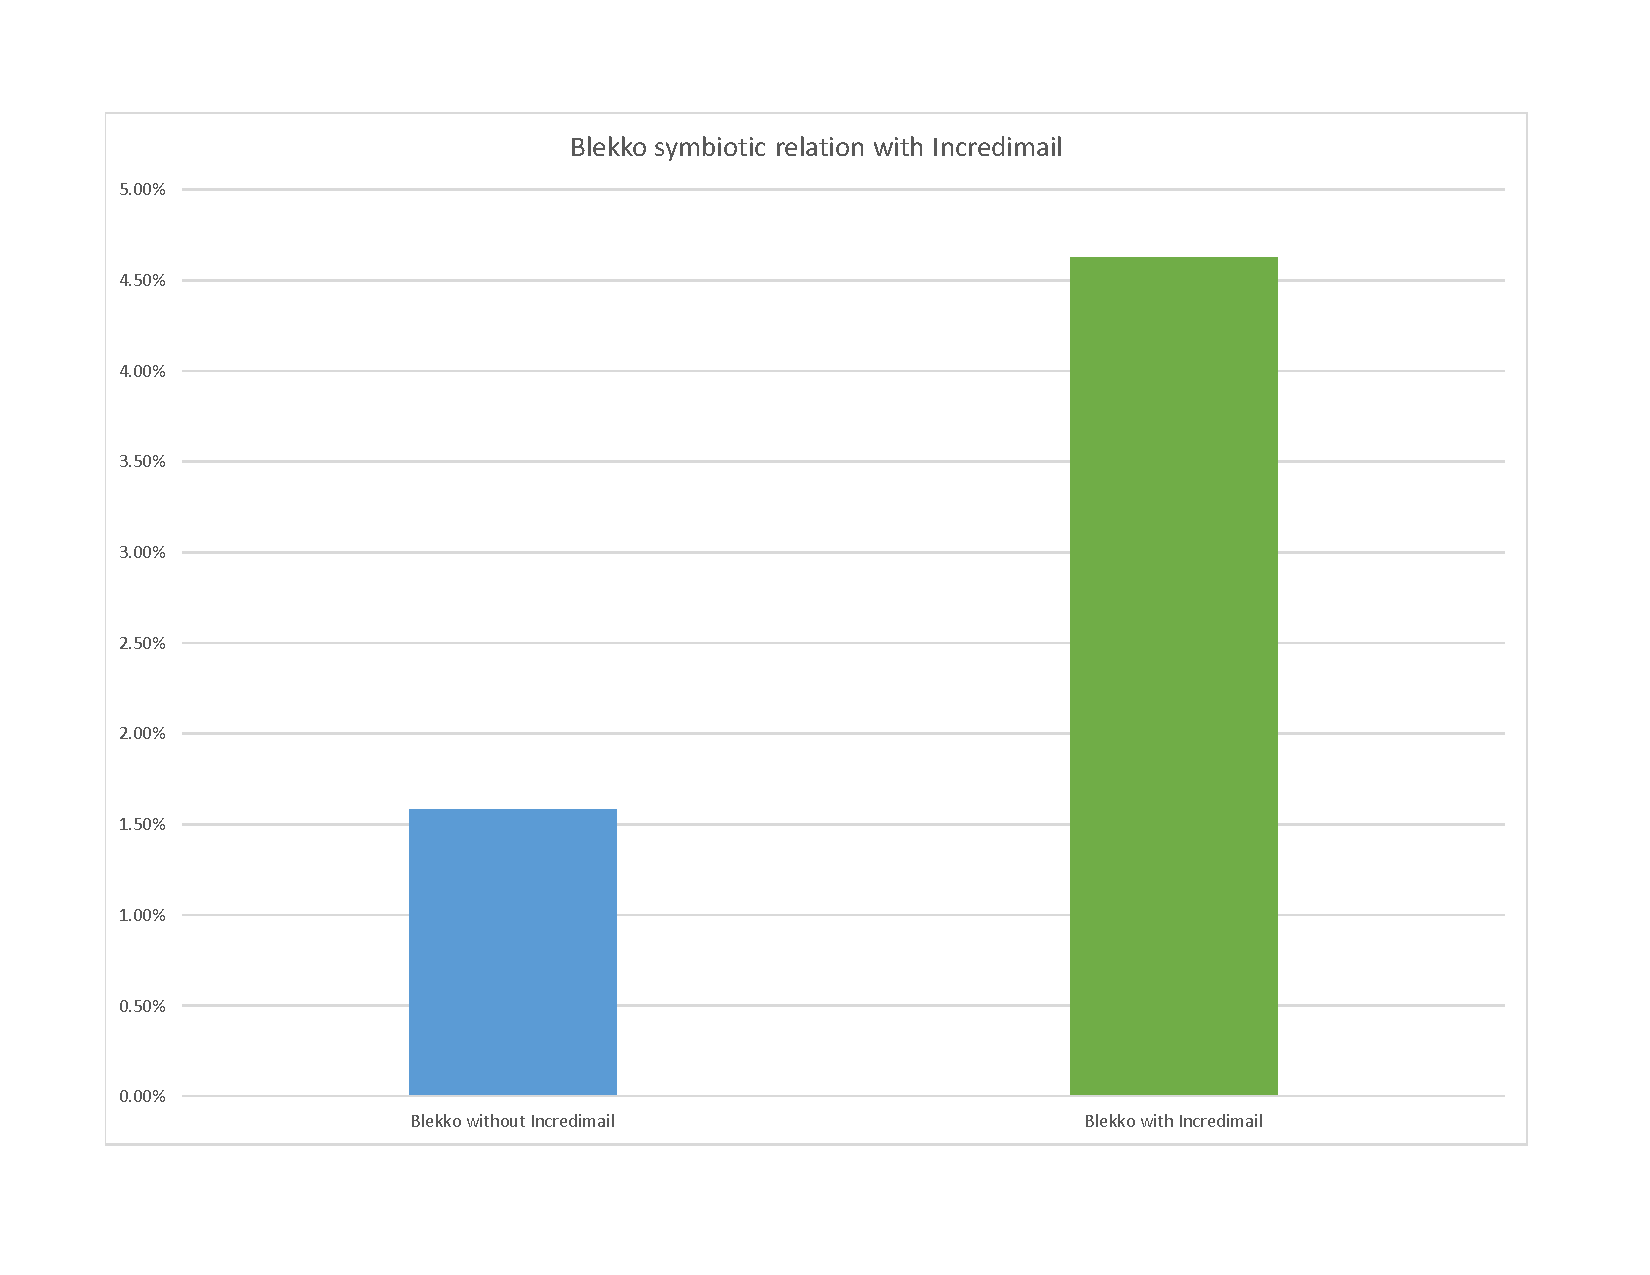
\includegraphics[width=\linewidth]{figures/blekko_sym_incredi.pdf}
\caption{Blekko symbiotic relationship with Incredimail}
\label{fig:blekko_sym_incredi}
\end{figure}

[RON: how is the following related to our results?]

It is well known that some company addons are getting to a user machine through "bundling" with addons of other companies. We see evidence of this in our results. For example, Ask Toolbars are integrated with Java downloads\footnote{\url{https://java.com/en/download/faq/ask_toolbar.xml}}. During the installation of Java, users are presented with an option of downloading an Ask Toolbar, see \autoref{fig:ask_offer}.
\begin{figure}[h]
\centering

\includegraphics[scale=.8,angle=0]{figures/ask_offer.png}
\caption{Bundled ASK Toolbar installation}
\label{fig:ask_offer}
\end{figure}


\subsection{Clash Relationships}
\label{sec:clash_relations}

In \autoref{sec:symb_relations}, we investigated symbiotic relationships between addon species, i.e. when one species benefit from another. Here, we will look for the opposite type of relationship. We can call it \emph{clash}, i.e. where one species benefits and causes harm to the other species, but we are referring to this relation as a clash between two (or more) species. The idea that lays in the way of of identifying clash relation is very similar to the way described in \autoref{sec:symb_relations}, again we are looking at the aggregated company scores, but this time we are looking for a company which score is getting lower when other company is present. In \autoref{fig:clash_pagerank}, you can see two examples for this relationship. The \autoref{fig:avira_clash_imesh} shows that when AntiVirus company Avira is present in ecosystem it causes an iMesh company to perform worth than in regular ecosystem. The same is shown in \autoref{fig:conduit_clash_hotspot}, between Conduit and Hotspot Shield company.

\begin{figure}[h]
\centering
\begin{subfigure}[b]{0.49\textwidth}
	\centering
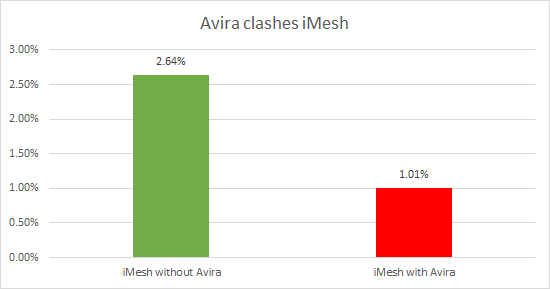
\includegraphics[scale=0.49]{figures/clashAviraImesh.png}
\caption{Avira clash relationship with iMesh}
\label{fig:avira_clash_imesh}
\end{subfigure}
\begin{subfigure}[b]{0.49\textwidth}
	\centering
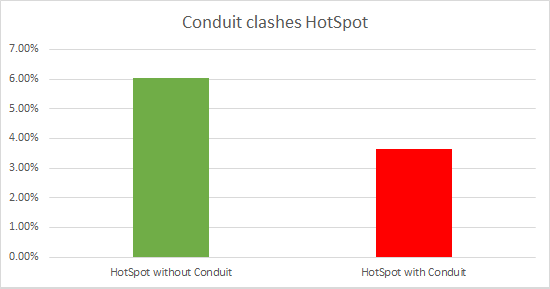
\includegraphics[scale=0.49]{figures/clashConduitHotSpot.png}
\caption{Conduit clash relationship with HotSpot}
\label{fig:conduit_clash_hotspot}
\end{subfigure}
\caption{Clash relationship between companies}
	\label{fig:clash_pagerank}
\end{figure}

Interesting validation for these measures could be applied if we would know about actual clash between companies from the \autoref{table:pagerank_scores} list. Having AntiVirus companies at the list comes handy, it is known that in most case two AV software programs can not exist on the same computer. Thus, using our terminology, the AV companies should have a clash relationship. And indeed, as shown in \autoref{fig:clash_av}, our algorithm detects AV companies as clashing.

\begin{figure}[h]
\centering
\begin{subfigure}[b]{0.49\textwidth}
	\centering
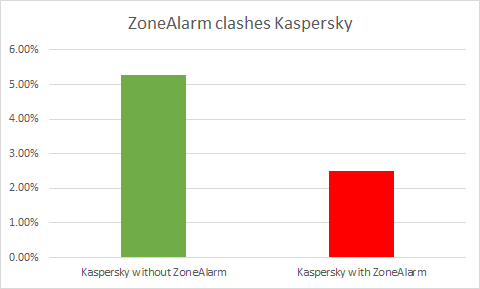
\includegraphics[scale=0.49]{figures/zone_clash_kaspersky.png}
\caption{ZoneAlarm clash relationship with Kaspersky}
\label{fig:zone_clash_kaspersky}
\end{subfigure}
\begin{subfigure}[b]{0.49\textwidth}
	\centering
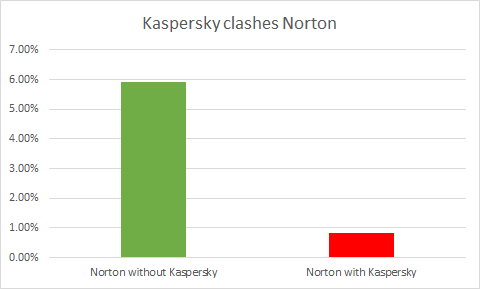
\includegraphics[scale=0.49]{figures/kaspersky_clash_norton.png}
\caption{Kaspersky clash relationship with Norton}
\label{fig:kaspersky_clash_norton}
\end{subfigure}
\caption{Clash relationship between AntiVirus companies}
	\label{fig:clash_av}
\end{figure}

\iffalse
After aggregating all add-ons for each for every company we have looked for what have happened to other company add-ons when PPR origin is a specific company.
For example, we have looked at HotSpot company and the impact it has on other companies.\\
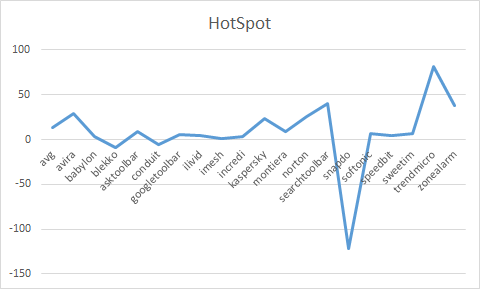
\includegraphics[scale=1.0]{hotspot.png}\\
As we can see from the chart some companies like trendmicro has a symbiosis with hotspot add-ons. While other companies, like SnapDo, are clashing with HotSpot add-ons.
This analysis, is even more interesting in light of recent security breach with Superfish and Komodia. After this security breach was identified, security researches where looking for more companies that have cooperated with Komodia. We believe that given that data, our algorithm would identify these companies as having a symbiosis with Komodia.
\fi

\iffalse
First, we needed some basic ranking of all add-ons from all companies, we believe that regular PageRank scores on this graph provide a good base line to all add-ons metrics. [Why do we need basic rankings? - RON][SELA] Basic ranking it is actually a baseline ranks, we were running a regular pagerank for this. It was used as a baseline, afterwards, for comparing how the rank of company addons has increased/decreased. BTW, this text is not in the thesis...
Then, we identified add-ons belonging to a company by looking for the company's name in addon descriptions. But what if the addon does not contain the company's name, can we still identify it as related to the company? To solve this problem, we applied an approach similar to the one we used to identify a "missing" addon. We ran PPR from all known add-ons of a specific company (for example, Babylon), and looked at all add-ons that drastically improved its rank compared to its previous rank given by PageRank.
By searching the addon names in the Web, many of them were found to be related to the company that originated the PPR (whose add-ons composed the PPR vector). For example,an  addon named tbmyba.dll, jumped from the 1200 rank position to the 15 rank position when running PPR from Babylon, and indeed we found that this addon is related to Babylon. 
After identifying all company add-ons, we decided to remove add-ons that are installed at fewer than 100 users' machines: these add-ons seemed to have almost no impact on the results but have made more difficult to look for tendencies between firms. [Why is that? - RON] [SELA] There were many addons that was installed only on few machines, we wanted to try to look at the addons "manually" and understand what is going on. Since the addons on small amount of machines did not have any impact, we could just remove them.\\
\fi


\section{Discussion}
We are comparing for each company its total weighted rank in PageRank with its total weighted rank in Personalized PageRank when another company is the PPR vector.
We have found that there are companies that co-exist well with other companies, there are even companies that improve greatly other companies add-ons rank.
We have also observed companies that cause other companies add-ons decline.



%\bibliographystyle{alpha}
\newpage
\appendix
\chapter{} 
\renewcommand{\figurename}{Appendix}

\begin{figure}[h]
\centering
\begin{subfigure}[b]{0.49\textwidth}
	\centering
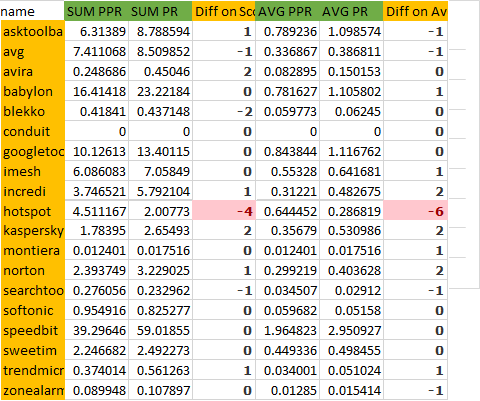
\includegraphics[scale=0.49]{figures/conduit_pr_scores.png}
\end{subfigure}
\begin{subfigure}[b]{0.49\textwidth}
	\centering
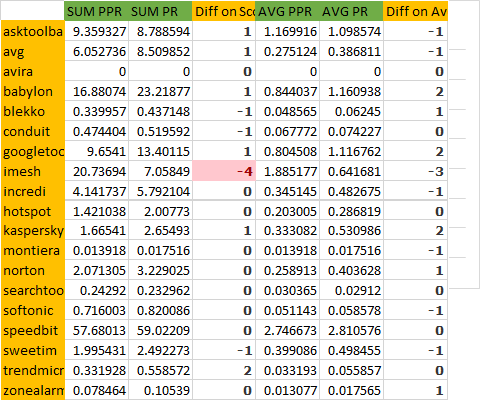
\includegraphics[scale=0.49]{figures/avira_pr_scores.png}
\end{subfigure}
\caption{PR scores}
	\label{fig:appendix_pr}
\end{figure}

\begin{figure}[h]
\centering
\begin{subfigure}[b]{0.49\textwidth}
	\centering
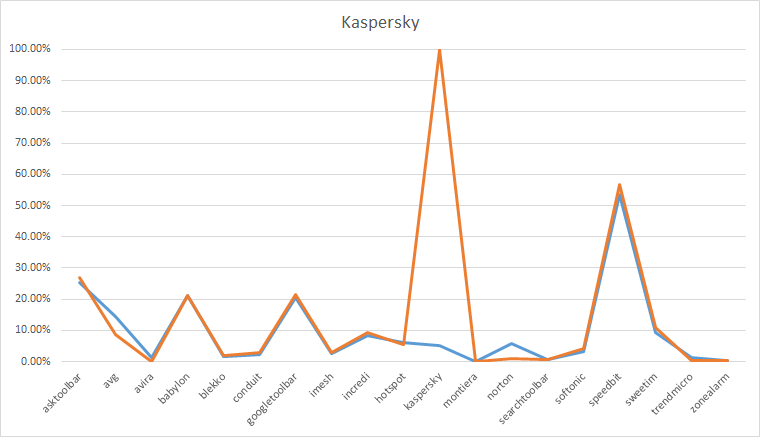
\includegraphics[scale=0.49]{figures/kaspersky_graph.png}
\end{subfigure}
\begin{subfigure}[b]{0.49\textwidth}
	\centering
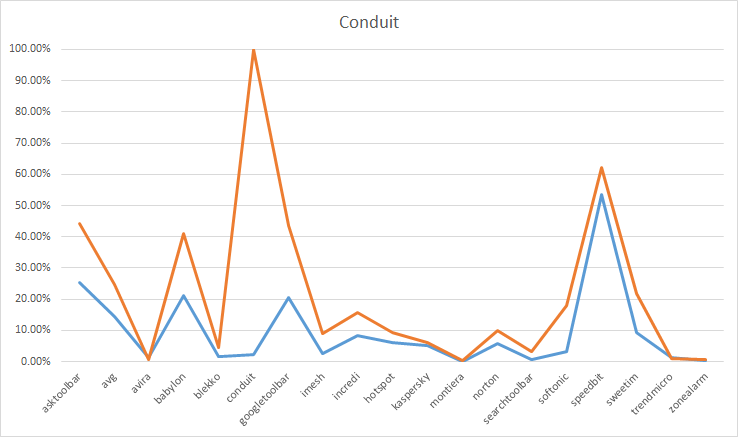
\includegraphics[scale=0.49]{figures/conduit_graph.png}
\end{subfigure}
\caption{Graph scores}
	\label{fig:appendix_pr}
\end{figure}

\begin{figure}[h]
\centering
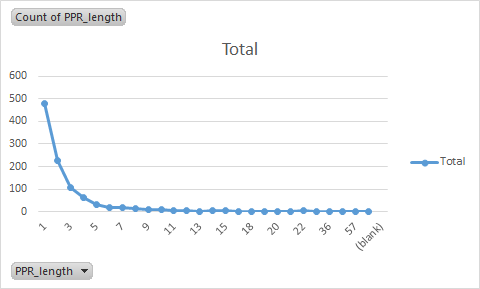
\includegraphics[scale=0.8]{figures/PPR_length_dist.png}
\caption{Personaliztion vector length}
\end{figure}



\bibliographystyle{apalike}
\bibliography{thesisdraft}
\addcontentsline{toc}{chapter}{Bibliography}

\end{document}

